\documentclass[a4paper, 11pt]{scrreprt}

%%%%%%%%%%%%%%%%%%%%%%%%%%%%%%%%%%%%%%%%%%%%%%%%%%%%%%%%%%%%%%%%%%%%%%%%%%%%
% Some common includes. Add additional includes you need.
%%%%%%%%%%%%%%%%%%%%%%%%%%%%%%%%%%%%%%%%%%%%%%%%%%%%%%%%%%%%%%%%%%%%%%%%%%%%
\RequirePackage[ngerman]{babel}
\RequirePackage[utf8]{inputenc}
\RequirePackage[T1]{fontenc}
\RequirePackage[margin=23mm,bottom=30mm]{geometry}
\RequirePackage{graphicx}
\RequirePackage{amsmath,amsfonts,amssymb,amsthm}
\RequirePackage{listingsutf8}
\RequirePackage{textcomp}
\RequirePackage{tikz}
\RequirePackage{eurosym}
\usetikzlibrary{snakes}

\linespread{1.25}


\usepackage{subfigure}
\usepackage{url}
\usepackage{pdfpages}

\usepackage{algorithm}
\usepackage[noend]{algpseudocode}


\usepackage{cite}
%\usepackage{multirow, tabularx}
%\usepackage{subcaption}


%%%%%%%%%%%%%%%%%%%%%%%%%%%%%%%%%%%%%%%%%%%%%%%%%%%%%%%%%%%%%%%%%%%%%%%%%%%%
% Defines for mathematical notation. Add additional defines as needed.
%%%%%%%%%%%%%%%%%%%%%%%%%%%%%%%%%%%%%%%%%%%%%%%%%%%%%%%%%%%%%%%%%%%%%%%%%%%%
\def\O{\mathcal{O}}
\def\sort{\mathrm{sort}}
\def\scan{\mathrm{scan}}
\def\dist{\mathrm{dist}}

%% Theorem, Lemma undso
\theoremstyle{plain} %Text ist Kursiv
\newtheorem{theorem}{Satz}[chapter]
\newtheorem{lemma}[theorem]{Lemma}
\newtheorem{proposition}[theorem]{Proposition}
\newtheorem{corollary}[theorem]{Korollar}

\theoremstyle{definition} %Text ist \"upright"
\newtheorem{remark}[theorem]{Bemerkung}
\newtheorem{definition}[theorem]{Definition}
\newtheorem{example}[theorem]{Beispiel}


%% wozu das ?! 
%\usepackage{listings}% http://ctan.org/pkg/listings
%\lstset{
%  basicstyle=\ttfamily,
%  mathescape,
%    showspaces=false,
%  showstringspaces=false
%}

%\lstset{
%   basicstyle=\fontsize{10}{13}\selectfont\ttfamily
%}

%\lstset{literate=%
%  {Ö}{{\"O}}1
%  {Ä}{{\"A}}1
%  {Ü}{{\"U}}1
%  {ß}{{\ss}}1
%  {ü}{{\"u}}1
%  {ä}{{\"a}}1
%  {ö}{{\"o}}1
%}

%\newcommand{\tomorrow}{{\AdvanceDate[1]\today}}


%%%%%%%%%%%%%%%%%%%%%%%%%%%%%%%%%%%%%%%%%%%%%%%%%%%%%%%%%%%%%%%%%%%%%%%%%%%%
%%%%% Titel DEFINITION!
%%%%%%%%%%%%%%%%%%%%%%%%%%%%%%%%%%%%%%%%%%%%%%%%%%%%%%%%%%%%%%%%%%%%%%%%%%%%

%\titlehead{\centering Bachelorarbeit mit dem Thema}

%\title{Bachelorarbeit mit dem Thema \\ ~}

%\subtitle{ Implementierung und experimentelle Untersuchung von Parallelem Global-Curveball zur Randomisierung
%Massiver Bipartiter Graphen\\ ~}
%\author{Marius Hagemann \\ 5732742 \\ s2486252@stud.uni-frankfurt.de \\~}
%\date{\tomorrow}
%\publishers{Betreuer: Prof. Dr. Ulrich Meyer \\ ~ \\ Goethe-Universität Frankfurt am Main \\ Fachbereich Informatik }

%\swapnumbers


%%%%%%%%%%%%%%%%%%%%%%%%%%%%%%%%%%%%%%%%%%%%%%%%%%%%%%%%%%%%%%%%%%%%%%%%
%%%%%   DEFINE MAKROS
%%%%%%%%%%%%%%%%%%%%%%%%%%%%%%%%%%%%%%%%%%%%%%%%%%%%%%%%%%%%%%%%%%%%%%%%

\newcommand{\SorSor}{\textbf{SortSort}}
\newcommand{\SorSea}{\textbf{SortSearch}}
\newcommand{\SeaSor}{\textbf{SearchSort}}
\newcommand{\SetSea}{\textbf{SetSearch}}
\newcommand{\SeaSet}{\textbf{SearchSet}}
\newcommand{\USetSea}{\textbf{USetSearch}}
\newcommand{\SeaUSet}{\textbf{SearchUSet}}
\newcommand{\perm}{\textbf{Permutation}}
\newcommand{\distr}{\textbf{Distribution}}
\newcommand{\true}{\textbf{true}}
\newcommand{\false}{\textbf{false}}

\newcommand{\gc}{Global Curveball}
\newcommand{\ct}{Curveball-Tausch}
\newcommand{\cb}{Curveball}

\newcommand{\partvek}{Partitions-Array}


\newcommand{\la}{large}
\newcommand{\sm}{small}
\newcommand{\fr}{fraction}


\newcommand{\nk}{NetworKit }
\newcommand{\cpp}{C++ }

\newcommand{\red}[1]{\textcolor{red}{\textbf{#1}}}
\newcommand{\blue}[1]{\textcolor{blue}{#1}}
\newcommand{\fett}[1]{\textbf{#1}}



\begin{document}
	
%%%%%%%%%%%%%%%%%%%%%%%%%%%%%%%%%%%%%%%%%%%%%%%%%%%%%%%%%%%%%%%%%%%%%%%%
%%%%%   TITELSEITE
%%%%%%%%%%%%%%%%%%%%%%%%%%%%%%%%%%%%%%%%%%%%%%%%%%%%%%%%%%%%%%%%%%%%%%%%

\begin{titlepage}
	\centering
	{\LARGE Bachelorarbeit mit dem Thema\par}
	%\vspace{1.5cm}
	\vfill
	{\huge\bfseries Implementierung und experimentelle Untersuchung 
					von Parallelem Global-Curveball zur Randomisierung
					Massiver Bipartiter Graphen\par}
	\vspace{2.5cm}
	{\Large verfasst von: \par}
	\vspace{1cm}
	{\LARGE \scshape Marius Hagemann\par}
	\vspace{0.5cm}
	{\large Matrikelnummer 5732742 \\ marius@ing-hagemann.de}
	\vfill
	{\Large \today}
	\vfill
	{\LARGE Betreuer:\\ Prof. Dr. Ulrich Meyer \\ Manuel Penschuck\par}
	\vspace{1.5cm}
	{\LARGE Goethe-Universität Frankfurt am Main \\ ~\\ Fachbereich Informatik}
\end{titlepage}

%\maketitle
\cleardoublepage 
\thispagestyle{empty}

\newpage
\section*{}

%%%%%%%%%%%%%%%%%%%%%%%%%%%%%%%%%%%%%%%%%%%%%%%%%%%%%%%%%%%%%%%%%%%%%%%%
%%%%%   ERKLÄRUNG + Inhaltsverzeichnis
%%%%%%%%%%%%%%%%%%%%%%%%%%%%%%%%%%%%%%%%%%%%%%%%%%%%%%%%%%%%%%%%%%%%%%%%


\includepdf[pages=1]{include/erkabschlbachelorinf}

\newpage

\tableofcontents



%%%%%%%%%%%%%%%%%%%%%%%%%%%%%%%%%%%%%%%%%%%%%%%%%%%%%%%%%%%%%%%%%%%%%%%%
%%%%%   ABSTRACT
%%%%%%%%%%%%%%%%%%%%%%%%%%%%%%%%%%%%%%%%%%%%%%%%%%%%%%%%%%%%%%%%%%%%%%%%


%\begin{abstract}
\chapter*{Abstract}


~\\

Ziel dieser Bachelorarbeit ist es, einen effizienten Algorithmus
zur Randomisierung massiver bipartiter Graphen zu entwickeln.
Die Graph Randomisierung ist vor allem zur Analyse von großen Netzwerken eine häufig verwendete Methode.
 Dazu 
wurde das Konzept des \gc{} auf bipartiten Graphen
angepasst. Es werden verschiedene Algorithmen zur Umsetzung diskutiert.
Anhand von Benchmarks wird unter den getesteten Methoden diejenige ausgewählt,
welche die geringste Laufzeit aufweist.
Im Vergleich zu dem schon existierenden \cb{} Algorithmus 
wird mit dem in dieser Arbeit entwickelten Algorithmus 
auf manchen Testinstanzen ein Speedup von bis zu 17 auf einem Prozessor mit 8 Kernen und Hyperthreading 
erreicht. Selbst ohne Parallelisierung wird mit einer sequenziellen Version des bipartiten \gc{} ein Speedup
von bis zu 2 gegenüber \cb{} erreicht.



%\end{abstract} 



%%%%%%%%%%%%%%%%%%%%%%%%%%%%%%%%%%%%%%%%%%%%%%%%%%%%%%%%%%%%%%%%%%%%%%%%
%%%%%   EINLEITUNG
%%%%%%%%%%%%%%%%%%%%%%%%%%%%%%%%%%%%%%%%%%%%%%%%%%%%%%%%%%%%%%%%%%%%%%%%


\chapter{Einleitung}
%%%%%%%%%%%%%%%%%%%%%%%%%%%%%%%%%%%%%%%%%%%%%%%%%%%%%%%%%%%%%%%%%%%%%%%%
%%%%%%%% Einleitung
%%%%%%%%%%%%%%%%%%%%%%%%%%%%%%%%%%%%%%%%%%%%%%%%%%%%%%%%%%%%%%%%%%%%%%%%
\glqq Bei der Analyse komplexer Netzwerke, wie beispielsweise sozialer Netzwerke, 
werden die zugrunde liegenden Graphen häufig mit zufälligen Graphen verglichen, 
um deren Struktur zu untersuchen.\grqq\footnote{frei übersetzt aus \cite{DBLP:conf/esa/CarstensH0PTW18} Abschntt 1}
Zum Erzeugen von zufälligen Graphen gibt es verschiedene Modelle wie beispielsweise der Erdos-Renyi-Graph \cite{erdos}
oder der Gilbert-Graph \cite{gilbert}.
\red{Diesen beiden Methoden ...?} 
Dabei haben aber die erstellten Graphen kaum eine Ähnlichkeit zu dem zu analysierenden Netzwerk.
Deshalb sind meist Zufallsgraphen gesucht, die zu einem gegebenen Graphen eine identische Gradsequenz
besitzen. Im Zufallsgraph soll also jeder Knoten den selben Grad haben wie im originalen Graph.
Ein Algorithmus, der diese Eigenschaft erfüllt ist beispielsweise Curveball \cite{curveball}.
Dabei wird ein Graph \glqq randomisiert, indem eine Sequenz an lokalen Modifikationen ausgeführt wird\grqq{}\footnote{frei übersetzt aus \cite{penschuck2020recent} Abschitt 6.4}
Diese lokalen Modifikationen werden als \ct{} bezeichnet. Bei einem \ct{} werden von zwei zufälligen 
Knoten die disjunkten Nachbarschaften durchgetauscht. Damit bleiben die Knotengrade unverändert.
Um den Graph zu randomisieren, werden einige von diesen \ct{en} hintereinander ausgeführt.
Um sicherzugehen, dass alle Knoten Teil eines \ct{es} gewesen sind, werden auf diese Weise
\glqq in Erwartung $\Theta(n\log(n))$  \ct{e} benötigt\grqq \footnote{frei übersetzt aus \cite{DBLP:conf/esa/CarstensH0PTW18} Abschitt 3.3}\red{. wohin mit dem punkt?}
Deswegen \red{wurde} eine Erweiterung namens \gc{} \cite{DBLP:conf/esa/CarstensH0PTW18} eingefügt. 
Für einen \gc{} Tausch werden 
\red{mehrere} \ct{e} nacheinander ausgeführt, sodass möglichst jeder Knoten Teil eines Tausches ist. 
\\
\\
Ziel dieser Bachelorarbeit ist es, \gc{} für bipartite Graphen anzupassen. Dazu werden gewisse 
Eigenschaften von bipartiten Graphen ausgenutzt, sodass Teile des originalen \gc{} Algorithmus
vereinfacht werden können. Ebenfalls ist es möglich einzelne \ct{e} parallel auszuführen.
Auf diese Weise soll eine deutlich geringere Laufzeit im Vergleich zu dem ursprünglichen \gc{}
Algorithmus erreicht werden.
Der neu entwickelte Algorithmus wird unter dem Namen \texttt{BipartiteGlobalCurveball} 
Teil vom Open-Source Projekt \nk{} werden.
\\
\\
Zu Beginn dieser Arbeit werden die wichtigsten Begriffe und mathematischen Grundlagen definitiert.
Im Anschluss werden verschiedenen Methoden, \gc{} umzusetzen,  besprochen und \red{ unter theorethischen
Aspekten verglichen.} 
Mit Hilfe von Benchmark Tests, wird schließlich die Methode ausgewählt, welche die geringste Laufzeit 
benötigt.


%\begin{itemize}
%\item wozu Randomisierung?
%-- Als (zufällige) Eingabe um Algorithmen zu testen?
%-- Zum Analysieren von Netzwerken?
%\red{bla}
%\item es gibt auch andere Methoden um zufällige Graphen zu erstellen (zufällige Kanten zwischen Knoten)
%aber dann bleibt die gewollte Struktur nicht erhalten
%also Global Curveball (, bei dem Kanten getauscht werden)
%\item wir beschränken uns hier nur auf den Spezialfall der bipartiten Graphen wodurch es einfacher wird ...?
%\item wozu GlobalCurveball?
%\item warum macht man das?
%\item-- Zufällige Graphen, wobei die Grade aller Knoten erhalten bleiben
%\item
%Was ist networkit? +  Quelle
%\item
%was heißt massiver graph ? 
%hoher Knotengrad??
%\end{itemize}


%%%%%%%%%%%%%%%%%%%%%%%%%%%%%%%%%%%%%%%%%%%%%%%%%%%%%%%%%%%%%%%%%%%%%%%%
%%%%%   Grundlagen
%%%%%%%%%%%%%%%%%%%%%%%%%%%%%%%%%%%%%%%%%%%%%%%%%%%%%%%%%%%%%%%%%%%%%%%%


\chapter{Grundlagen}



%%%%%%%%%%%%%%%%%%%%%%%%%%%%%%%%%%%%%%%%%%%%%%%%%%%%%%%%%%%%%%%%%%%%%%%%
%%%%%% Definitionen
%%%%%%%%%%%%%%%%%%%%%%%%%%%%%%%%%%%%%%%%%%%%%%%%%%%%%%%%%%%%%%%%%%%%%%%%

\section{Mathematische Definitionen}
Zu Beginn definieren wir die grundlegenden mathematischen Begriffe. Als wichtigste Grundlage dient 
hierbei das Konstrukt des \red{ungerichteten} Graphen.
\begin{definition}[Graph] ~\\
Ein (ungerichteter) \textbf{Graph} $G = (V,E)$ ist ein Tupel bestehend aus einer Knotenmenge $V$ und einer Kantenmenge
 $E$. Eine Kante verbindet zwei Knoten miteinander und ist damit eine Menge, aus zwei Knoten.
 Es gilt: $E \subseteq \{ \{u,v\} |\ u,v \in V, u \neq v \}$.  
\end{definition}
\red{In dieser Arbeit} spielt eine spezielle Klasse von Graphen, bipartite Graphen, eine zentrale Rolle.
Bei einem bipartiten Graphen kann man die Knoten in zwei Mengen teilen, sodass alle Kanten nur zwischen den 
beiden Mengen verlaufen und nicht innerhalb einer Menge. Formal bedeutet dies:
\begin{definition}[bipartiter Graph] ~\\
Ein Graph $G=(V,E)$ heißt \textbf{bipartit}, wenn es Teilmengen $V_1 \subset V$ und $V_2 \subset V$ gibt, für die 
$V_1 \cup V_2 = V$ und $V_1 \cap V_2 = \emptyset$ gilt,
 sodass für jede Kante $e \in E$ ein $u \in V_1$ und ein $v \in V_2$ existiert, sodass $e = \{u,v\}$ gilt.
Die Knotenmengen $V_1$ und $V_2$ werden auch als Partitionen bezeichnet.
\end{definition}

\noindent
Ein Beispiel für einen bipartiten Graphen sieht man in Abbildung \ref{fig:bipstd}. Dabei gilt für die Partitionen:
$V_1 = \{v_1,v_2,v_3,v_4\}$ und $V_2 = \{v_5,v_6,v_7,v_8\}$. Man sieht deutlich, dass alle Kanten die Partitionen
$V_1$ und $V_2$ ''kreuzen''.

\begin{figure}[h]
%bipartiter graph
\centering
\begin{tikzpicture}
\tikzset{node style/.style={shape=circle,draw=black, inner sep=5pt,}}
                                
\node[node style] at (0, 0)     (1)     {$v_1$};
\node[node style] at (0, -1.5)   (2)     {$v_2$};
\node[node style] at (0, -3)     (3)     {$v_3$};
\node[node style] at (0, -4.5)   (4)     {$v_4$};

\node[node style] at (3, 0)     (5)     {$v_5$};
\node[node style] at (3, -1.5)   (6)     {$v_6$};
\node[node style] at (3, -3)   (7)     {$v_7$};
\node[node style] at (3, -4.5)   (8)     {$v_8$};

   
\draw[line width=0.1mm, >=latex]
            (1)     edge[right]    node {} (5)
            (1)     edge[right]    node {} (6)
            (1)     edge[right]    node {} (7)
            (2)     edge[right]    node {} (5)
            (2)     edge[right]    node {} (6)
            (3)     edge[right]    node {} (6)
            (4)     edge[right]    node {} (5)
            (4)     edge[right]    node {} (8)
;
\end{tikzpicture}
\caption{Beispiel eines bipartiten Graphen}
\label{fig:bipstd}
\end{figure}
\red{überleitung}
Für einen \ct ist vor allem der Begriff der Nachbarschaft, genauer der gemeinsamen und disjunkten 
Nachbarschaft, entscheidend.
\begin{definition}[Nachbarschaft]~\\
Ein Knoten $u \in V$ heißt \textbf{benachbart} (oder \fett{adjazent}) zu einem 
anderen Knoten $v \in V$, wenn es eine Kante $\{u,v\} \in E $ gibt. Die Menge $N(u)$ aller adjazenten Knoten
von $u$ nennt man \fett{Nachbarschaft}.
\end{definition}
\begin{definition}[gemeinsame und disjunkte Nachbarschaft]~\\
	Die \fett{gemeinsame} Nachbarschaft $N_{c}(u,v)$ zweier Knoten $u$ und $v$ ist die Menge aller Knoten, die sowohl
	zu $u$ als auch zu $v$ adjazent sind. In der \fett{disjunkten} Nachbarschaft $N_{d}(u,v)$ von $u$ und $v$ sind dagegen 
	alle Knoten die nur zu einem der beiden Knoten adjazent sind. \\
	Es gilt also $N_{c}(u,v) = N(u) \cap N(v)$ und $N_{d}(u,v) = \big(N(u) \cup N(v)\big)\setminus \big(N(u) \cap N(v) \big)$
\end{definition}
\red{Dabei bemerken wir, dass in einem Bipartiten Graphen zwei Knoten aus einer Partitionsklasse nie\dots\dots
}
\begin{definition}[Knotengrad]~\\
Der \fett{Grad} eines Knotens $v \in V$ wird mit $\deg(v)$ bezeichnet und entspricht die Anzahl
der adjazenten Knoten von $v$. Es gilt also $\deg(v) = |N(v)|$ für alle Knoten $v\in V$.

\end{definition}
\begin{definition}[Gradsequenz]~\\
Die \fett{Gradsequenz} eines Graphen $G = (V,E)$ mit $|V| = n$ Knoten ist gegeben durch das Tupel
$D = (d_{1}, \dots, d_{n})$, wobei $d_{i} = \deg(v_{1})$ der Grad des Knotens $v_{i}$ ist.
\end{definition}
\red{in abbildung ... hat man grade soundso, sequenz so}





%%%%%%%%%%%%%%%%%%%%%%%%%%%%%%%%%%%%%%%%%%%%%%%%%%%%%%%%%%%%%%%%%%%%%%%%
%%%%%% NetworKit
%%%%%%%%%%%%%%%%%%%%%%%%%%%%%%%%%%%%%%%%%%%%%%%%%%%%%%%%%%%%%%%%%%%%%%%%
\section{\nk}

\nk \cite{nk} ist ein Open-Source Projekt, dass es zum Ziel hat, ''Werkzeuge für die
Analyse großer Netzwerke, in den Größenordnungen von Tausenden bis Milliarden 
von Kanten, zur Verfügung zu stellen''.
\footnote{aus \cite{nk} abgerufen am 10.2.2020}
\\
Innerhalb von \nk Gibt es einfache Graph Datenstrukturen \red{blabla}
\\
Man kann es mit python nutzen \red{blabla}





%%%%%%%%%%%%%%%%%%%%%%%%%%%%%%%%%%%%%%%%%%%%%%%%%%%%%%%%%%%%%%%%%%%%%%%%
%%%%%% Datenstruktur
%%%%%%%%%%%%%%%%%%%%%%%%%%%%%%%%%%%%%%%%%%%%%%%%%%%%%%%%%%%%%%%%%%%%%%%%

\section{Datenstruktur}
In \nk \red{\cite{nk} muss das immer hin, wenn \nk erwähnt wird?!} werden Graphen in einer eigenen Datenstruktur gespeichert. Um den Algorithmus 
zu vereinfachen, wird der Graph in eine einfachere Datenstruktur transformiert. Dazu erstellen wir 
eine Art Adjazenzlistendarstellung des Graphen, wobei jedoch keine echten verketteten
Listen verwendet werden, sondern lediglich Vektoren. 
Es wird also für einen Knoten
$v \in V$ ein Vektor erstellt, indem alle adjazenten Knoten gespeichert sind.
Da wir ausschließlich bipartite Graphen betrachten werden, speichern wir noch in 
einem weiteren Vektor die Knoten von einer der beiden Bipartitionsklassen \red{die größere?}.
\\
Die Vektoren sind dabei vom C++ Datentyp \texttt{std::vector}.

\red{WAS muss die Datenstruktur können? -- Zwei Knoten zufällig auswählen, -- Nachbarschaften berechenen -- 
Nachbarn tauschen--}


%%%%%%%%%%%%%%%%%%%%%%%%%%%%%%%%%%%%%%%%%%%%%%%%%%%%%%%%%%%%%%%%%%%%%%%%
%%%%%% Global Curveball
%%%%%%%%%%%%%%%%%%%%%%%%%%%%%%%%%%%%%%%%%%%%%%%%%%%%%%%%%%%%%%%%%%%%%%%%

\section{Global Curveball \red{(auf bipartiten Graphen)}}
Wie \red{in der Einleitung beschrieben}, ist \gc ein Verfahren zum Randomisieren von Graphen.
Dabei ist als Eingabe ein beliebiger bipartiter Graph gegeben, der in einen \red{anderen/zufälligen}
Graph mit äquivalenter Gradsequenz transformiert werden soll.
\\
Die Aufgabe ist also, bei einer gegebenen Gradsequenz $D$, eine uniform verteilte \red{Stichprobe???}
aus der Menge aller Graphen mit Gradsequenz $D$ zurückzugeben. Durch das Ausführen von \gc 
bleibt also für jeden Knoten $v\in V$ sein Grad $\deg(v)$ erhalten. \red{(aus survey übernommen)}
\\
\\



~\\
\\
\\\
\\


\gc ist eine Variante vom ETCTS kp..

gradsequenz

MARKOV
äääöööÄÖ

%%%%% CURVEBALL TRADE auf graph
\begin{figure}[h]
\centering
\begin{tikzpicture}
		\tikzset{node style/.style={shape=circle,draw=black, inner sep=5pt,}}
                                
\node[node style] at (0, -0.75)     (1)     {$v_1$};
\node[node style] at (0, -2.25)   (2)     {$v_2$};


\node[node style, fill=gray] at (3, 0)     (5)     {$v_3$};
\node[node style, fill=yellow] at (3, -1.5)   (6)     {$v_4$};
\node[node style, fill=yellow] at (3, -3)   (7)     {$v_5$};


   
\draw[line width=0.1mm, >=latex]
            (1)     edge[right]    node {} (5)
            (1)     edge[right]    node {} (7)
            (2)     edge[right]    node {} (5)
            (2)     edge[right]    node {} (6)

;
\end{tikzpicture}
\hspace{2cm}
\begin{tikzpicture}
\tikzset{node style/.style={shape=circle,draw=black, inner sep=5pt,}}
                                
\node[node style] at (0, -0.75)     (1)     {$v_1$};
\node[node style] at (0, -2.25)   (2)     {$v_2$};

\node[node style, fill=gray] at (3, 0)     (5)     {$v_3$};
\node[node style, fill=yellow] at (3, -1.5)   (6)     {$v_4$};
\node[node style, fill=yellow] at (3, -3)   (7)     {$v_5$};


\draw[line width=0.1mm, >=latex]
            (1)     edge[right]    node {} (5)
            (1)     edge[right]    node {} (6)
            (2)     edge[right]    node {} (5)
            (2)     edge[right]    node {} (7)

;
\end{tikzpicture}
\caption{Beispiel eines Curveball-Tausches}
\label{fig:curveball_trade_graph}
	
\end{figure}



%%%%% CURVEBALL TRADE auf Vektor
\begin{figure}[h]
\centering
  \begin{tikzpicture}[decoration=brace]
      
      
    %% COMMON FÄRBEN  
    \foreach \x in {0,1,2,3}
		{
			\fill [ fill =gray, draw =black ]  (\x ,0) rectangle (\x+1 ,1) ;
			\fill [ fill =gray, draw =black ]  (\x ,-1.5) rectangle (\x+1 ,-0.5) ;
		};

    %% DISJOINT OBEN FÄRBEN  
    \foreach \x in {4,5,6,7,8,9}
		{
			\fill [ fill =yellow, draw =black ]  (\x ,0) rectangle (\x+1 ,1) ;
		};
		
	%% DISJOINT UNTEN FÄRBEN  
    \foreach \x in {4,5,6,7,8,9,10,11,12}
		{
			\fill [ fill =yellow, draw =black ]  (\x ,-1.5) rectangle (\x+1 ,-0.5) ;
		};
    
    
    
    % untere geschweifte Klammer mit Text darunter:
    \draw[decorate, yshift=-1ex] (3.8,-1.5) -- node[below=0.4ex] {gemeinsame Nachbarschaft} (0.2,-1.5);
    \draw[decorate, yshift=-1ex] (12.8,-1.5) -- node[below=0.4ex] {disjunkte Nachbarschaft} (4.2,-1.5);


	\draw[bend left=80, <->,>=latex, very thick] (8.5,0.5) to  node[right= 3ex] {vertauschen} (10.5,-1) ;

  \end{tikzpicture}
  \caption{Beispiel für einen Curveball-Tausch}
  \label{fig:curveball_trade_vector}
  
\end{figure}




\red{Wir betrachten wie die einzelnen cb trades ausgeführt werden...}






%%%%%%%%%%%%%%%%%%%%%%%%%%%%%%%%%%%%%%%%%%%%%%%%%%%%%%%%%%%%%%%%%%%%%%%%
%%%%%% Parallelität
%%%%%%%%%%%%%%%%%%%%%%%%%%%%%%%%%%%%%%%%%%%%%%%%%%%%%%%%%%%%%%%%%%%%%%%%

\section{Parallelisierung}

\red{OPENMP UND SO...}


%\begin{itemize}
%\item \textbf{Notation}, Graph, bipartitheit, randomisierung, ...? 
%\item theoretische grundlagen
%\item beweis, kanten Tauschen wird uniform verteilt... (markov ??) FDSM sequenz -> algo macht komischen Graph draus -> 
%\item Kanten tauschen, globaler Tausch, zufall
%\item Parallelität (OpenMP)?
%\item networkit (was ist das, wofür braucht man das
%\end{itemize}




%%%%%%%%%%%%%%%%%%%%%%%%%%%%%%%%%%%%%%%%%%%%%%%%%%%%%%%%%%%%%%%%%%%%%%%%
%%%%%   Implementierung
%%%%%%%%%%%%%%%%%%%%%%%%%%%%%%%%%%%%%%%%%%%%%%%%%%%%%%%%%%%%%%%%%%%%%%%%


\chapter{Implementierung eines \ct{es} }
Wie bereits in Kapitel \ref{sec:global_curveball} erwähnt, muss die disjunkte Nachbarschaft
der beiden Knoten $u$ und $v$ bekannt sein, um einen \ct{} auf diesen Knoten $u$ und $v$
auszuführen. Der \ct{} besteht dann darin, diese Knoten aus $N_{d}(u,v)$ zu durchmischen.
Deshalb beschäftigen wir uns zuerst damit wie man die disjunkte Nachbarschaft bestimmt.

%%%%%%%%%%%%%%%%%%%%%%%%%%%%%%%%%%%%%%%%%%%%%%%%%%%%%%%%%%%%%%%%%%%%%%%%
%%%%%% COMMON NEIGHBORS
%%%%%%%%%%%%%%%%%%%%%%%%%%%%%%%%%%%%%%%%%%%%%%%%%%%%%%%%%%%%%%%%%%%%%%%%

\section{Bestimmung der disjunkten Nachbarschaft}
\label{sec:common}
Gesucht sind alle Knoten aus der disjunkten Nachbarschaft der Knoten $u$ und $v$.
Nach der Definition \ref{def:common_disjoint} liegt jeder Knoten aus den Nachbarschaften $N(u)$ und $N(v)$ 
entweder in der disjunkten oder in der gemeinsamen Nachbarschaft. Das Ziel besteht also darin, 
für jeden Knoten aus $N(u) \cup N(v)$ zu entscheiden, ob er zu $N_{d}(u,v)$ oder $N_{c}(u,v)$ gehört.
\\

Die Nachbarschaften $N(u)$ und $N(v)$ liegen --- wie in Abschnitt 
\ref{sec:datenstruktur} beschrieben --- jeweils
in einem Array vor. Der Übersichtlichkeit 
wegen werden wir die beiden
Arrays ebenfalls mit $N(u)$ und $N(v)$ bezeichnen. Aufgabe ist es,
 für jedes Element aus den beiden Arrays zu entscheiden,
ob es entweder in beiden Arrays vorkommt oder nur in einem von den beiden. Dafür 
gibt es verschiedene algorithmische Ansätze.
\\

Als ersten naiven Ansatz könnte man für jedes Element des Arrays $N(u)$ das gesamte andere 
Array $N(v)$ per linearer Suche nach diesem Element durchsuchen. Hierfür ergibt sich eine Laufzeit von
$\O(|N(u)|\cdot|N(v)|)$. Dies ist aber nicht sinnvoll, da wir 
im Falle von massiven Graphen davon ausgehen können, dass die Arrays (also die Nachbarschaften)
 groß werden. 
\\

Dieses Problem kann man beispielsweise verhindern, indem man beide Arrays aufsteigend sortiert. 
Um herauszufinden,
welche Werte in beiden Arrays vorkommen, muss man lediglich $N(u)$ und $N(v)$ gleichzeitig linear durchlaufen
und testen, ob die Werte gleich sind oder nicht. Somit muss man jedes 
Element der beiden Arrays --- nach dem Sortieren --- 
nur einmal betrachten, was offensichtlich zu einer verbesserten Laufzeit im Vergleich zum naiven
Ansatz führt. Man erhält damit eine Laufzeit von $\O(|N(u)|\cdot \log (|N(u)|)  + |N(v)|\cdot\log(|N(v)|))$. 
Diese Variante wird im Folgenden als \SorSor{} bezeichnet. 
\\

Die Laufzeit hängt dabei im Wesentlichen vom Sortieren ab. Daher führen wir eine Variante ein, 
die wir \fett{vorsortiert} nennen. Bei dieser Variante nehmen wir an, dass
die Arrays immer im sortierten Zustand vorliegen. Somit würde bei \SorSor{} das Sortieren wegfallen
und man müsste die beiden Arrays nur noch linear durchlaufen, was zu einer Laufzeit von $\O(|N(u)| + |N(v)|)$
führen würde. 
Es ist jedoch nicht offensichtlich, dass die Variante zu einer insgesamt besseren Laufzeit eines
\ct{es} führt, da ein \ct{} schließlich auch noch aus dem Durchmischen der disjunkten Nachbarschaft besteht.
Dadurch könnte die \red{Vorsortierheit} verletzt werden, weshalb man am Ende des \ct{es} nochmal sortieren
muss, um sie wieder aufrecht zu erhalten. Ob das \red{Vorsortieren} zu einem Vorteil führt, wird in Kapitel 
\ref{cap:tests} anhand von Laufzeitmessungen geklärt.
\\

Die Variante \SorSor{} lässt sich leicht abwandeln, indem wir nur eines der beiden Arrays sortieren.
Auf diese Weise können wir die Laufzeit des einen Sortiervorgangs sparen. Sortieren
wir das größere Array (ohne Beschränkung der Allgemeinheit $N(v)$), bezeichnen wir die Variante als \SorSea{}. Um zu erkennen, 
welche Elemente zur gemeinsamen und welche zur disjunkten Nachbarschaft gehören, kann man für jeden
Knoten aus $N(u)$ per binärer Suche in logarithmischer Zeit prüfen, ob der Knoten auch in $N(v)$ vorhanden ist.
Damit ergibt sich eine Laufzeit von $\O(|N(v)| \cdot \log(|N(v)|) + |N(u)| \cdot \log(|N(v)|)$. Analog dazu
nennen wir die Variante, in der das kleinere Array sortiert wird, \SeaSor. 
Auch hier könnte die vorsortiert Invariante einen Vorteil bringen.
\\

Eine weitere Methode, um viele Werte schnell zu durchsuchen, bietet die Datenstruktur \texttt{set}, welche
einem binären Suchbaum entspricht, beispielsweise eines Rot-Schwarz-Baums.
Dabei wird jedes Element des einen Arrays in den Suchbaum eingefügt. 
Für jedes Element des anderen Arrays kann nun in logarithmischer
Zeit bestimmt werden, ob es im \texttt{set} und somit auch im ursprünglichen Array vorhanden ist.
Somit erhält man die identischen asymptotischen Laufzeiten wie bei der Verwendung der
binären Suche. Je nach Implementierung des Suchbaums könnte es aber auch zu einer verbesserten
Laufzeit führen. 
Für diese Möglichkeit gibt es ebenfalls zwei 
analoge Varianten, nämlich \SetSea, bei der die Elemente des größeren Arrays in das \texttt{set} eingefügt werden
und \SeaSet, bei der das kleinere Array zum \texttt{set} hinzugefügt wird.
Auch bei diesen beiden Optionen könnte es sinnvoll sein, wenn die vorsortiert Invariante aufrechterhalten wird.
Dies hängt ebenfalls von der internen Implementierung des Suchbaums ab.
\\

Die letzte Methode, die wir an dieser Stelle betrachten werden,
ist die Verwendung der Datenstruktur \texttt{unordered\_set}. Diese ist \texttt{set} sehr ähnlich, jedoch mit
dem Unterschied, dass die Werte nicht in geordneter Reihenfolge gespeichert werden, sondern
in einer Hash-Tabelle. Ein Vorteil einer Hash-Tabelle liegt darin, 
dass das Einfügen und Suchen von Elementen
erwartet in konstanter Zeit erfolgt.
Ebenfalls gibt es hierbei wieder die Varianten, 
in denen entweder das größere Array in das \texttt{unordered\_set} eingefügt wird (\USetSea) 
oder das kleinere (\SeaUSet).{}
Asymptotisch ergibt sich in beiden Fällen eine \underline{erwartete} Laufzeit von $\O(|(N(u)| + |N(v)|)$.
Diese Laufzeit hängt jedoch stark von der Implementierung und dem Füllgrad  der Hash-Tabelle ab. 
Schließlich werden wir auch bei den letzten beiden Methoden prüfen,
 ob die Invariante eventuell zu einer besseren Laufzeit führt.
\\

Zusammenfassend betrachten wir also insgesamt sieben verschiedene Möglichkeiten, um die disjunkte
und gemeinsame Nachbarschaft zu berechnen. Für jede dieser Varianten prüfen wir zusätzlich,
ob die vorsortiert Invariante zu einer verbesserten Laufzeit führt oder ob es sich
nicht lohnt, diese aufrechtzuerhalten.


%%%%%%%%%%%%%%%%%%%%%%%%%%%%%%%%%%%%%%%%%%%%%%%%%%%%%%%%%%%%%%%%%%%%%%%%
%%%%%% Nachbarn Tauschen
%%%%%%%%%%%%%%%%%%%%%%%%%%%%%%%%%%%%%%%%%%%%%%%%%%%%%%%%%%%%%%%%%%%%%%%%

\section{Tauschen der Nachbarn}
\label{sec:trade}
Im vorherigen Teil wurde beschrieben, wie man die gemeinsame und die disjunkte Nachbarschaft zweier Knoten
$u$ und $v$ bestimmt. Nun beschäftigen wir uns damit, wie man die Knoten der disjunkten Nachbarschaft zufällig tauscht. Als Eingabe 
stehen die Arrays $N_{d}(u,v)$, welches alle Knoten aus der disjunkten Nachbarschaft enthält
und $N_{c}(u,v)$, das die gemeinsamen Nachbarn enthält, zur Verfügung. Weiterhin seien $\text{deg}(u)$ und
$\text{deg}(v)$ die ursprünglichen Knotengrade. Zusätzlich definieren wir uns die Mengen
$D_{u} = N_{d}(u,v) \cap N(u)$, in der die disjunkten Nachbarn von Knoten $u$ liegen, 
und $D_{v} = N_{d}(u,v) \cap N(v)$, in der die disjunkten Nachbarn von $v$ liegen. Die anfänglich
leeren Arrays, in denen die Ausgabe --- also die neuen Nachbarschaften von $u$ und $v$ --- zurückgegeben 
werden soll, bezeichnen wir wieder als $N(u)$ und $N(v)$.
Wir betrachten zwei unterschiedliche Möglichkeiten.
\\

Die erste Idee besteht darin,  
das Array der disjunkten Nachbarschaft zufällig zu permutieren, sodass jedes Element an 
einer zufälligen Position steht. Um nun die beiden \glqq neuen\grqq{} Nachbarschaften von $u$ und $v$ zu erstellen,
werden zuerst die Knoten aus der gemeinsamen Nachbarschaft in die leeren Arrays $N(u)$ und $N(v)$ kopiert.
Dann werden die ersten $D_{u}$ Elemente aus dem permutierten Array in $N(u)$ kopiert, die restlichen
in $N(v)$. Somit haben die Nachbarschaften durch den Tausch ihre ursprüngliche Größe nicht verändert, es gilt $|N(u)| = \deg(u)$ und
$|N(v)| = \deg(v)$.
Zur besseren Veranschaulichung ist in Abbildung \ref{fig:trade_shuffle} ein Beispiel zu sehen.
\begin{figure}
\centering
  \begin{tikzpicture}[decoration=brace]
    % Die Grundlinie:
    \draw(0,0)--(10,0);
    \draw(0,1)--(10,1);

    % Striche und Beschriftung in Abständen 0, 2, 4, 6, ...
    \foreach \x/\xtext in {0,1,2,3,4,5,6,7,8,9,10}
      \draw(\x,0)--(\x,1) node[below] {};
      
    % untere geschweifte Klammer mit Text darunter:
    \draw[decorate, yshift=-1ex] (3.8,0) -- node[below=0.4ex] {$D_{u}$} (0.2,0);

    \draw[decorate, yshift=-1ex] (9.8,0) -- node[below=0.4ex] {$D_{v}$} (4.2,0);

\node[] at (-1.2, 0.5)     (5)     {$N_{d}(u,v):$};

  \end{tikzpicture}
  \caption{Beispiel für einen Tausch mit der Variante \perm. Dabei wird das Array der 
  disjunkten Nachbarschaft $N_{d}(u,v)$ zufällig permutiert. Die ersten $D_{u}$ Elemente werden der Nachbarschaft
  von $u$ zugeordnet, die restlichen $D_{v}$ zur Nachbarschaft von $v$. }
  \label{fig:trade_shuffle}
\end{figure}
Bei diesem Verfahren fällt  jedoch auf, dass einige Elemente beim Permutieren unnötig vertauscht werden.
Für jedes Element ist es eigentlich nur entscheidend, ob es unter den ersten $D_{u}$  liegt (also zum Array
$N(u)$ hinzugefügt wird) oder nicht. Auf welcher Position es genau in 
diesen Bereichen liegt, ist nicht von Relevanz. Ohne Beschränkung der Allgemeinheit gelte 
$N(u) \le N(v)$. Dann kann man
also die Laufzeit dieser Variante verbessern, indem nicht das ganze Array der disjunkten Nachbarschaft zufällig permutiert 
wird, sondern nur die ersten $D_{u}$ Elemente zufällig gewählt werden.
 Dies setzt die Funktion 
\texttt{random\_bipartition\_shuffle} um.
\\

Ein Nachteil dieser Methode besteht jedoch darin, dass durch das zufällige Vertauschen die beiden resultierenden Arrays
$N(u)$ und $N(v)$ im Allgemeinen nicht mehr sortiert sind. Damit wird die im Abschnitt \ref{sec:common} beschriebene
Invariante eventuell verletzt. Möchte man die Invariante aufrechterhalten, müssen somit die beiden Arrays
in einem letzten Schritt nochmals sortiert werden.
Wir nennen diese Variante \perm.
\\

Die zweite Möglichkeit, die wir betrachten, werden wir als \distr{} bezeichnen.
Die Idee besteht dabei, dass wir über jedes Element des Arrays $N_{d}(u,v)$ iterieren und eine Wahrscheinlichkeit
berechnen, mit
der das Element in die Nachbarschaft von $u$ (beziehungsweise $v$) eingefügt werden soll. Dann wird in einem 
Bernoulli Experiment mit genau dieser Wahrscheinlichkeit ein Zufallsbit gezogen. Je nachdem welchen
Wert das Zufallsbit hat, wird das Element dann entweder in $N(u)$ oder in $N(v)$ kopiert. Dies wird so lange
wiederholt bis eines der beiden Arrays seine maximale Kapazität erreicht hat. 
\\

Um die Wahrscheinlichkeit zu berechnen werden am Anfang zwei Variablen $n_u$ und $n_v$ initialisiert, 
welche den Kapazitäten der beiden Arrays $u$ und $v$ entsprechen, wenn die Elemente aus der 
gemeinsamen Nachbarschaft nicht berücksichtigt werden. Es gilt also $n_u = |D_{u}|$ und
$n_v= |D_{v}|$.
Damit hat das erste Element des Arrays $N_{d}(u,v)$ eine Wahrscheinlichkeit von $p_u = \frac{n_u}{n_u+n_v}$, dem
Array $N(u)$ hinzugefügt zu werden und analog eine Wahrscheinlichkeit $p_v = \frac{n_v}{n_u+n_v}$, um
in $N(v)$ zu gelangen. Offensichtlich gilt $p_u + p_v = 1$. Dann wird mit einer der beiden
Wahrscheinlichkeiten das Bernoulli Experiment durchgeführt, wobei es irrelevant ist, welche Wahrscheinlichkeit
man dazu wählt, da $p_u$ genau die Gegenwahrscheinlichkeit von $p_v$ ist und umgekehrt. 
Wählt man beispielsweise $p_u$ und das Experiment liefert eine eins, dann wird das aktuelle Element
in $N(u)$ kopiert. Dabei
hat sich aber offensichtlich die verbleibende Kapazität des Arrays $N(u)$ verringert. Also muss
der Wert $n_u$ dekrementiert werden. Dies gilt analog, falls das Element in die Nachbarschaft von $v$ kopiert wird.
Somit ändern sich nach jeder Iteration die Wahrscheinlichkeiten $p_u$ beziehungsweise $p_v$.
Gilt nach irgendeinem Zeitpunkt entweder $n_u = 0$ oder $n_v = 0$, steht offenbar in einem der Arrays 
keine freie Kapazität mehr zur Verfügung. Somit werden die übrigen Elemente, die noch in $N_{d}(u,v)$ vorhanden sind, 
einfach dem anderen Array hinzugefügt.
\\

An dieser Stelle  kann man jedoch noch eine Optimierung vornehmen.
Da bei dem Bernoulli Experiment die Wahrscheinlichkeit $p_{u}$ --- beziehungsweise $p_{v}$ --- eine
Dezimalzahl ist, werden zur Berechnung laufzeitintensive Gleitkommaoperationen 
benötigt. Um dies zu umgehen, kann man eine zufällige Ganzzahl aus dem Intervall
$[0, n_{u} + n_{v}-1]$ ziehen. Anschließend prüft man, ob die gezogene Zahl echt kleiner als $n_{u}$ ---
beziehungsweise $n_{v}$ ---
ist. Wenn dies der Fall ist, fährt man genauso fort, wie wenn das Bernoulli Experiment eine eins
zurückgibt. Auf diese Weise 
ergeben sich für ein Element die gleichen Wahrscheinlichkeiten in das jeweilige Array zu geraten, wie
beim Bernoulli Experiment. Dabei werden aber ausschließlich \red{Integer} Operationen verwendet, welche
von der Recheneinheit schneller verarbeitet werden können.
\\

\red{Dieses Vorgehen ist auch als Reservoir Sampling\cite{DBLP:journals/toms/Vitter85} bekannt.}
\\

Ein Vorteil dieser Methode ist, dass die in \ref{sec:common} beschriebene Invariante aufrecht erhalten werden kann.
War das Array der disjunkten Nachbarschaft vor Beginn dieser Methode aufsteigend sortiert,
dann sind auch die bisherigen Elemente der Arrays $N(u)$ und $N(v)$ aufsteigend sortiert, da für jedes
Element nacheinander entschieden wurde, ob es zur Nachbarschaft von $u$ oder von $v$ hinzugefügt wird und dabei die
Reihenfolge der Elemente untereinander nicht verändert wurde.
\\

Zum Schluss müssen noch die gemeinsamen Nachbarn zu den Arrays $N(u)$ und $N(v)$ hinzugefügt werden.
Möchte man die Invariante aufrecht erhalten, dann sind die beiden Arrays wie beschrieben schon
aufsteigend sortiert. Da auch die Elemente aus $N_{c}(u,v)$ aufsteigend sortiert sind, erhält man
die endgültigen Arrays von $N(u)$ und $N(v)$ durch ein Mergen mit $N_{c}(u,v)$. Soll die Invariante jedoch
nicht aufrecht erhalten werden, reicht es aus, die Elemente aus $N_{c}(u,v)$ jeweils an das Ende der beiden Arrays
zu kopieren.
\\

Wird die Variante vorsortiert nicht verwendet, ergibt sich für \perm{} und \distr{}
die gleiche asymptotische Laufzeit von $\O(|N(u)| + |N(v)|)$. 
Beim Verwenden der vorsortiert Variante ändert sich die asymptotische Laufzeit für \distr{}
nicht, da das Mergen ebenfalls in linearer Zeit ausgeführt werden kann. Bei \perm{}
hingegen müssen die beiden Arrays nochmals sortiert werden. Somit entsteht
eine Laufzeit von $\O(|N(u)| \cdot \log(|N(u)|) + |N(v)| \cdot \log(|N(v)|))$.


%%%%%%%%%%%%%%%%%%%%%%%%%%%%%%%%%%%%%%%%%%%%%%%%%%%%%%%%%%%%%%%%%%%%%%%%
%%%%%% Global Curveball Tausch
%%%%%%%%%%%%%%%%%%%%%%%%%%%%%%%%%%%%%%%%%%%%%%%%%%%%%%%%%%%%%%%%%%%%%%%%


\section{\ct}
Wie schon in Abschnitt \ref{sec:global_curveball} beschrieben, 
besteht ein Curveball Tausch auf zwei Knoten $u$ und $v$ daraus, die 
gemeinsame und disjunkte Nachbarschaft der beiden Vektoren zu bestimmen
und schließlich die Knoten aus der disjunkten Nachbarschaft zufällig zu tauschen.
\\
Die verschiedenen Methoden, die wir hierfür untersuchen werden, 
entstehen durch Kombination aller Varianten, die in \ref{sec:common} und \ref{sec:trade} beschrieben 
werden. Alle diese Möglichkeiten sind in der Tabelle \ref{tab:varianten} mit ihren jeweiligen asymptotischen
Laufzeiten zusammengefasst.


\begin{table}
	\centering
	\begin{tabular}{c||c|c||c|c}
		 & \multicolumn{2}{c||}{\distr} & \multicolumn{2}{c}{\perm} \\ \hline \hline
		\fett{vorsortiert} & \true & \false & \true & \false
		\\ \hline\hline
		%\SorSor & $\O(|N(u)| + |N(v)|)$ & $\O(|N(u)\cdot \log(|N(u)|) + |N(v)|\cdot \log(|N(v)|))$ & $\O(|N(u)| + |N(v)|)$ & \\ \hline
		\SorSor 	& $\O(l)$ 				& $\O(l\cdot \log(l))$ 		& $\O(l \cdot \log(l))$ 					& $\O(l\cdot \log(l))$ 	\\ \hline
		\SeaSor 	& $\O(l\cdot \log(s))$ 	& $\O(l\cdot  \log(s))$ 	& $\O(l\cdot  \log(l))$ 	& $\O(l\cdot  \log(s))$ \\ \hline
		\SorSea 	& $\O(s\cdot \log(l))$ 	& $\O(l\cdot  \log(l))$ 	& $\O(l\cdot  \log(l))$ 	& $\O(l\cdot  \log(l))$ \\ \hline
		\SeaSet 	& $\O(l\cdot \log(s))$ 	& $\O(l\cdot  \log(s))$ 	& $\O(l\cdot  \log(l))$ 	& $\O(l\cdot  \log(s))$ \\ \hline
		\SetSea 	& $\O(s\cdot \log(l))$ 	& $\O(l\cdot  \log(l))$ 	& $\O(l\cdot  \log(l))$ 	& $\O(l\cdot  \log(l))$ \\ \hline
		\SeaUSet	& $\O(l) \dagger$		& $\O(l) \dagger$ 			& $\O(l\cdot  \log(l))$ 	& $\O(l) \dagger$		\\ \hline
		\USetSea	& $\O(l) \dagger$ 		& $\O(l) \dagger$ 			& $\O(l\cdot  \log(l))$ 	& $\O(l) \dagger$
	\end{tabular}
	\caption{Jedes Feld in der Tabelle entspricht einer Variante für einen \ct{}.
	Dabei sind jeweils die asymptotischen Laufzeiten der Varianten gegeben. Zur besseren 
	Übersicht sind die Laufzeiten nicht in Abhängigkeit von $|N(u)|$ und $|N(v)|$ angegeben, 
	sondern in den Variablen $l$ und $s$, wobei $l$ der Größe des größeren Arrays entspricht und
	$s$ der Größe des kleineren. Es gilt also $l = \max\{|N(u)|,|N(v)|\}$ und $s = \min\{|N(u)|,|N(v)|\}$ und folglich $s = \O(l)$.
	Erwartete Laufzeiten sind dabei mit $\dagger$ markiert.}
	\label{tab:varianten}
\end{table}



%%%%%%%%%%%%%%%%%%%%%%%%%%%%%%%%%%%%%%%%%%%%%%%%%%%%%%%%%%%%%%%%%%%%%%%%
%%%%%% Ṕseudocode
%%%%%%%%%%%%%%%%%%%%%%%%%%%%%%%%%%%%%%%%%%%%%%%%%%%%%%%%%%%%%%%%%%%%%%%%


\section{Pseudocode}
Wie wir in Kapitel \ref{sec:entscheidung} sehen werden, 
hat die Variante mit den Methoden \SorSor{} und \distr{} und der genutzten vorsortiert
Invariante das beste Laufzeitverhalten. Deswegen gehen wir an dieser Stelle 
noch einmal genauer auf diese beiden Methoden ein, indem wir sie in Pseudocode
beschreiben. In Algorithmus \ref{algo:sortsort} ist \SorSor{} beschrieben, in Algorithmus \ref{algo:distr}
\distr.
\\

Bei beiden Varianten wird davon ausgegangen, dass die vorsortiert Invariante genutzt wird.
Somit fällt bei Algorithmus \ref{algo:sortsort} beispielsweise das anfängliche Sortieren weg.

\begin{algorithm}
  \caption{SortSort}\label{algo:sortsort}
  \begin{algorithmic}[1]
    \Procedure{SortSort}{$u,v$}
	  \State U $ \gets N(u)$ \Comment{vorsortierte Nachbarschaft von u}
	  \State V $ \gets N(v)$ \Comment{vorsortierte Nachbarschaft von v}
	  %\State
	  \State nu $\gets 0$ \Comment{Zähler für U}
	  \State nv $\gets 0$ \Comment{Zähler für V}
	  %\State disjoint $ \gets \emptyset$
	  %\State common $ \gets \emptyset$
      
      \While{(nu < |U|) and (nv < |V|)}
        \If{U[nu] < V[nv]}
			\State disjoint.\texttt{append(}U[nu]\texttt{)} \Comment{Füge das Element in disjoint ein}
			\State nu ++
			\ElsIf{U[nu] > V[nv]}
				\State disjoint.\texttt{append(}V[nv]\texttt{)} \Comment{Füge das Element in disjoint ein}
				\State nv ++
			\ElsIf{U[nu] == V[nv]}
				\State common.\texttt{append(}U[nu]\texttt{)} \Comment{Füge das Element in common ein}
				\State nu ++
				\State nv ++
        \EndIf
      \EndWhile
      \If{nu $\neq$ U.\texttt{size()}} \Comment{Die restlichen Elemente sind disjunkte Nachbarn}
			\State disjoint.\texttt{append(} U[nu], U[nu+1], \dots\texttt{)}
			\Else{}
			\State disjoint.\texttt{append(} V[nv], V[nv+1], \dots\texttt{)}
      \EndIf
      \State \textbf{return} common, disjoint
   \EndProcedure
  \end{algorithmic}
  \label{algo:sortsort}
\end{algorithm}



\begin{algorithm}
\begin{algorithmic}[1]
\Procedure{Distribution}{common, disjoint}
	\State nu $\gets$ U.\texttt{size()} - common.\texttt{size()} \Comment{Kapazität von $u$}
	\State nv $\gets$ V.\texttt{size()} - common.\texttt{size()} \Comment{Kapazität von $v$}
	\State i = 0
	\While{i < disjoint.\texttt{size()}}
		\State X $\sim \mathcal{B}(\frac{\text{nu}}{\text{nu}+\text{nv}})$  \Comment{Zufallsbit Bernoulli verteilt mit Wahrscheinlichkeit $\frac{nu}{nu+nv}$}

		\If{X==1}
			\State U.\texttt{append(}disjoint[i]\texttt{)} \Comment{Füge das Element in U ein}
			\State i++
			\State nu- - \Comment{aktualisiere die Kapazität}
		\Else{} 
			\State V.\texttt{append(}disjoint[i]\texttt{)}\Comment{Füge das Element in V ein}
			\State i++
			\State nv- -\Comment{aktualisiere die Kapazität}
		\EndIf{}
	\EndWhile{}	
	\State U.\texttt{merge(}common\texttt{)} \Comment{Merge U mit der gemeinsamen Nachbarschaft}
	\State V.\texttt{merge(}common\texttt{)} \Comment{Merge V mit der gemeinsamen Nachbarschaft}
	\State \textbf{return} U, V
\EndProcedure
\end{algorithmic}
	\caption{Distribution}
	\label{algo:distr}
\end{algorithm}














%%%%%%%%%%%%%%%%%%%%%%%%%%%%%%%%%%%%%%%%%%%%%%%%%%%%%%%%%%%%%%%%%%%%%%%%
%%%%%   Experimentelle Untersuchung
%%%%%%%%%%%%%%%%%%%%%%%%%%%%%%%%%%%%%%%%%%%%%%%%%%%%%%%%%%%%%%%%%%%%%%%%


\chapter{Experimentelle Untersuchung}
\label{cap:tests}
Wie im vorherigen Kapitel beschrieben, existieren verschiedene Varianten, einen \gc{} Tausch 
durchzuführen. Für das Finden der gemeinsamen Nachbarschaft betrachten wir sieben verschiedene Methoden, 
für das Tauschen der Nachbarschaft zwei. Weiterhin prüfen wir, ob es sinnvoll ist, 
die Variante der Vorsortierung zu nutzen oder nicht.
Kombiniert man all diese Möglichkeiten erhält man somit insgesamt 28 verschiedene Varianten einen \gc{} 
Tausch umzusetzen.
In diesem Kapitel diskutieren wir, welche der Varianten am geeignetsten ist.
%%%%%%%%%%%%%%%%%%%%%%%%%%%%%%%%%%%%%%%%%%%%%%%%%%%%%%%%%%%%%%%%%%%%%%%%
%%%%%% Aufbau
%%%%%%%%%%%%%%%%%%%%%%%%%%%%%%%%%%%%%%%%%%%%%%%%%%%%%%%%%%%%%%%%%%%%%%%%

\section{Versuchsaufbau}
Um die einzelnen Varianten auf ihre Laufzeit zu testen, wird ein Versuch aufgebaut.
Dazu werden alle Methoden in \cpp programmiert. Diese werden dann auf unterschiedlichen
Instanzen getestet und mittels Google Benchmark \cite{benchmark} wird die Zeit gemessen, 
die für das Ausführen benötigt wurde.
\\

Wie beschrieben benötigen die Methoden als Eingabe keinen Graph, 
sondern lediglich zwei Arrays, welche jeweils die Nachbarschaft zweier Knoten repräsentieren. Ohne 
Beschränkung der Allgemeinheit nennen wir das größere Array \fett{large}, das kleinere \fett{small}.
Um möglichst gut zu erkennen, wie sich die verschiedenen Methoden bei unterschiedlichen
Eingaben verhalten, messen wir die Laufzeiten für eine ganze Reihe an Instanzen. 
Um ein gutes Bild zu erhalten, sollten folgende Fälle abgedeckt sein:

\begin{itemize}
	\item Beide Arrays liegen in der gleichen Größenordnung
	
	\item Eines der Arrays ist wesentlich größer als das andere
	
	\item Der Anteil an gemeinsamen Elementen ist groß
	
	\item Der Anteil an gemeinsame Elementen  ist klein
\end{itemize}

Um dies zu erreichen, wird jedes Experiment in  mehreren Runden durchgeführt, in denen das Array large von anfänglich 128
Elementen auf bis zu 4.000.000 Elementen vergrößert wird. 
Jede Runde besteht aus mehreren Durchläufen, bei denen das Array small eine Größe zwischen 32 Elementen und der jeweiligen Größe von large hat.
Für jeden dieser Durchläufe werden die beiden Arrays mit zufälligen, aber paarweise verschiedenen
Werten befüllt, bis sie die entsprechende Größe haben. 
Dabei existiert jedoch kein Element, welches in beiden Arrays 
enthalten ist, was dazu führen würde, dass ein \gc{} 
Tausch nichts verändern würde. Um sicherzugehen,
dass die gemeinsame Nachbarschaft nicht leer ist, müssen somit Elemente des einen Arrays 
in das andere hineinkopiert werden. Damit die Größe der gemeinsamen Nachbarschaft
variiert wird, werden zuerst 10, dann 25, 50 und 75 Prozent der Elemente kopiert. 
\\

Eine einzelne Test-Messung lässt sich somit durch ein Tripel \fett{(\la, \sm, \fr)} beschreiben, wobei
large  und small für die Größe der jeweiligen Arrays stehen.
Der Wert \fett{\fr} steht dabei für den prozentualen Anteil der gemeinsamen Elemente an small.





%%%%%%%%%%%%%%%%%%%%%%%%%%%%%%%%%%%%%%%%%%%%%%%%%%%%%%%%%%%%%%%%%%%%%%%%
%%%%%% Messung
%%%%%%%%%%%%%%%%%%%%%%%%%%%%%%%%%%%%%%%%%%%%%%%%%%%%%%%%%%%%%%%%%%%%%%%%

\section{Messung}
\label{sec:messung}
Auf die im vorherigen Abschnitt beschriebene Weise werden die verschiedenen Instanzen erstellt und
mittels Google Benchmark die Zeit gemessen. Aus Zeitgründen werden jedoch nicht alle Werte 
für \la{} und \sm{} erstellt. Deshalb verdoppeln wir in jedem Schritt die Werte von \la{} und \sm{,}
anstatt sie um eins zu inkrementieren. Somit ergeben sich insgesamt 672 Instanzen, auf denen die Laufzeiten der 
einzelnen Methoden gemessen werden. 
Um Rauschen zu verringern, wird dabei jede Variante so oft wiederholt
 bis mindestens 100ms gemessen wurden.
Um eventuelle Messfehler zu minimieren, wird
dieser Vorgang jeweils fünf mal wiederholt. 
Als resultierender Messwert dient der Mittelwert dieser Wiederholungen.
\\

Alle Messungen wurden auf einem Rechner mit 64GB Arbeitsspeicher und einem Prozessor vom Typ Intel(R) Xeon(R) CPU E5-2630 v3 @ 2.40GHz,
mit 8 Kernen, Hyperthreading und einem Cache von 20 MB, ausgeführt.
Mit dieser Konfiguration hat die Dauer für alle 28 Varianten in Summe ungefähr 19 Stunden betragen.




%%%%%%%%%%%%%%%%%%%%%%%%%%%%%%%%%%%%%%%%%%%%%%%%%%%%%%%%%%%%%%%%%%%%%%%%
%%%%%% Auswertung
%%%%%%%%%%%%%%%%%%%%%%%%%%%%%%%%%%%%%%%%%%%%%%%%%%%%%%%%%%%%%%%%%%%%%%%%

\section{Auswertung}
\label{ref:auswertung}
Die ermittelten Messdaten werden schließlich mit Hilfe von 
Jupyter Notebook \cite{jupyter} ausgewertet. Dabei
handelt es sich um ein Tool, mit dem man Python-Programme auf einfache Art und Weise erstellen und 
ausführen kann.
Innerhalb von Python nutzen wir die Bibliotheken \fett{Matplotlib} und \fett{pandas}, um die Daten
zu analysieren und grafisch aufzuarbeiten.
\begin{figure}
\centering
	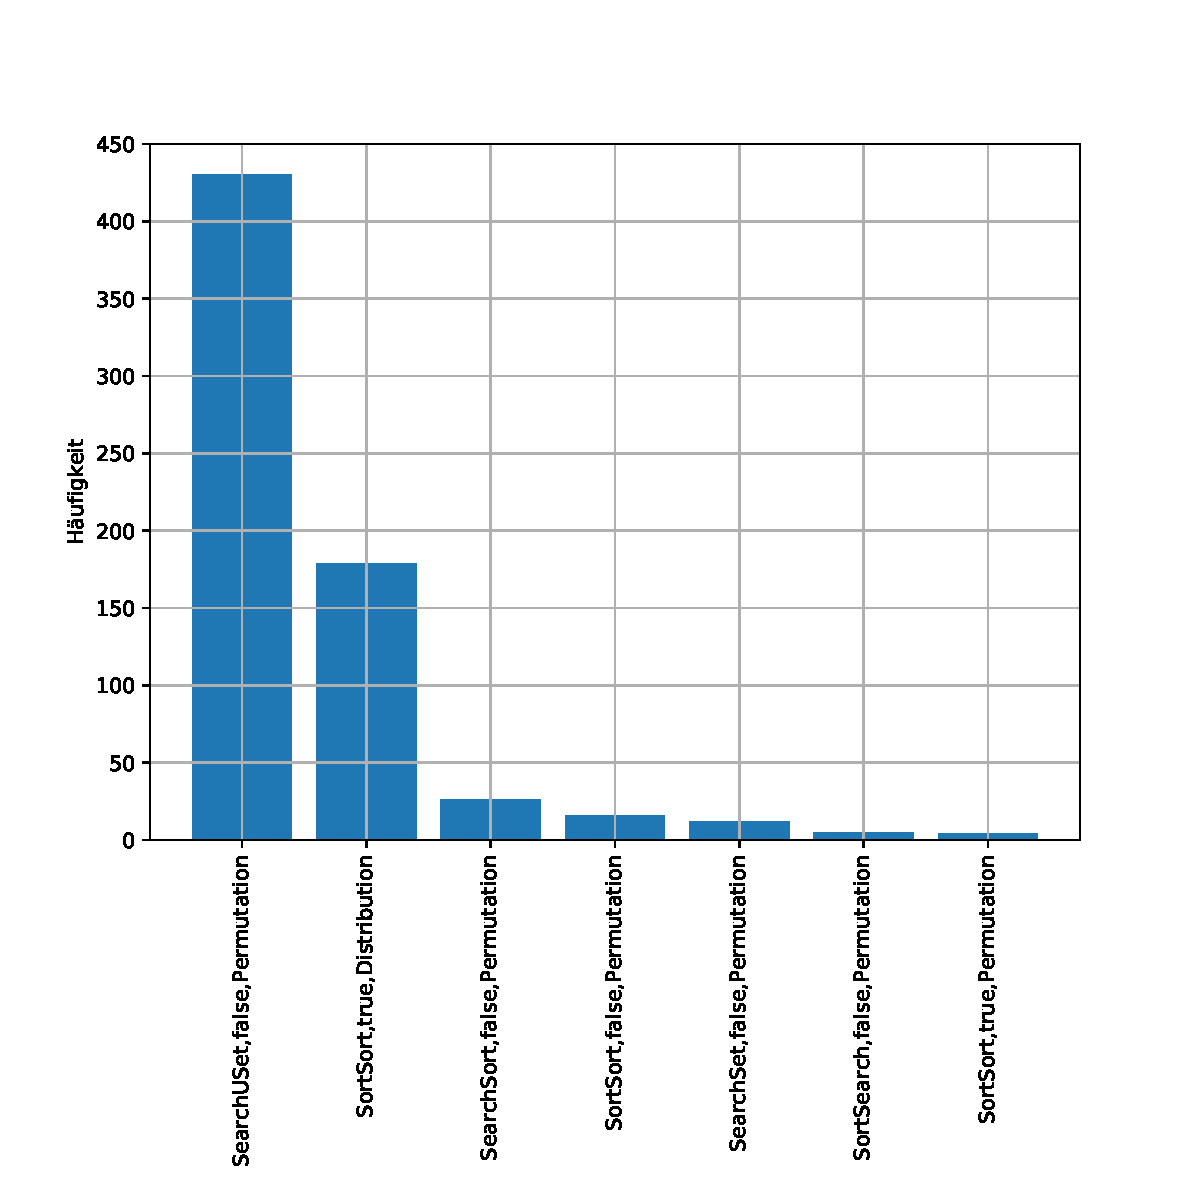
\includegraphics[width = 0.65\textwidth]{figures/counting.pdf}
	\caption{Vergleich der Varianten, welche am häufigsten die geringste Laufzeit aufweisen}
	\label{fig:messung_counting}
\end{figure}
\\

Zuerst betrachten wir für jede Instanz, welche Methode am schnellsten war.
Interessant sind dann jeweils die Methoden, für die häufig die geringste Laufzeit gemessen wurde.
In Abbildung \ref{fig:messung_counting} ist dazu ein Balkendiagramm dargestellt.
Dabei sieht man eindeutig, dass die Variante (\SeaUSet, \false, \perm) mit Abstand 
auf den meisten Instanzen die schnellste Laufzeit aller Methoden hat. Die
430 Instanzen auf welchen (\SeaUSet, \false, \perm) die schnellste Methode ist, entsprechen einem Anteil von rund
64\%. Mit 179 \glqq gewonnenen\grqq{} Instanzen folgt die Variante (\SorSor, \true, \distr), was einem Anteil von
27\% entspricht. Zusammen ist somit in etwa 91\% aller getesteter Instanzen eine dieser beiden Methoden
die Schnellste gewesen. Daher liegt der Schluss nahe, sich beim Suchen der \glqq besten\grqq{} Variante,
auf diese beiden Methoden zu beschränken. 
\\

Um nicht fälschlicherweise \glqq gute\grqq{} Methoden auszuschließen,
betrachten wir einen weiteren Plot in Abbildung \ref{fig:messung_slowdown}. 
\begin{figure}
\centering
	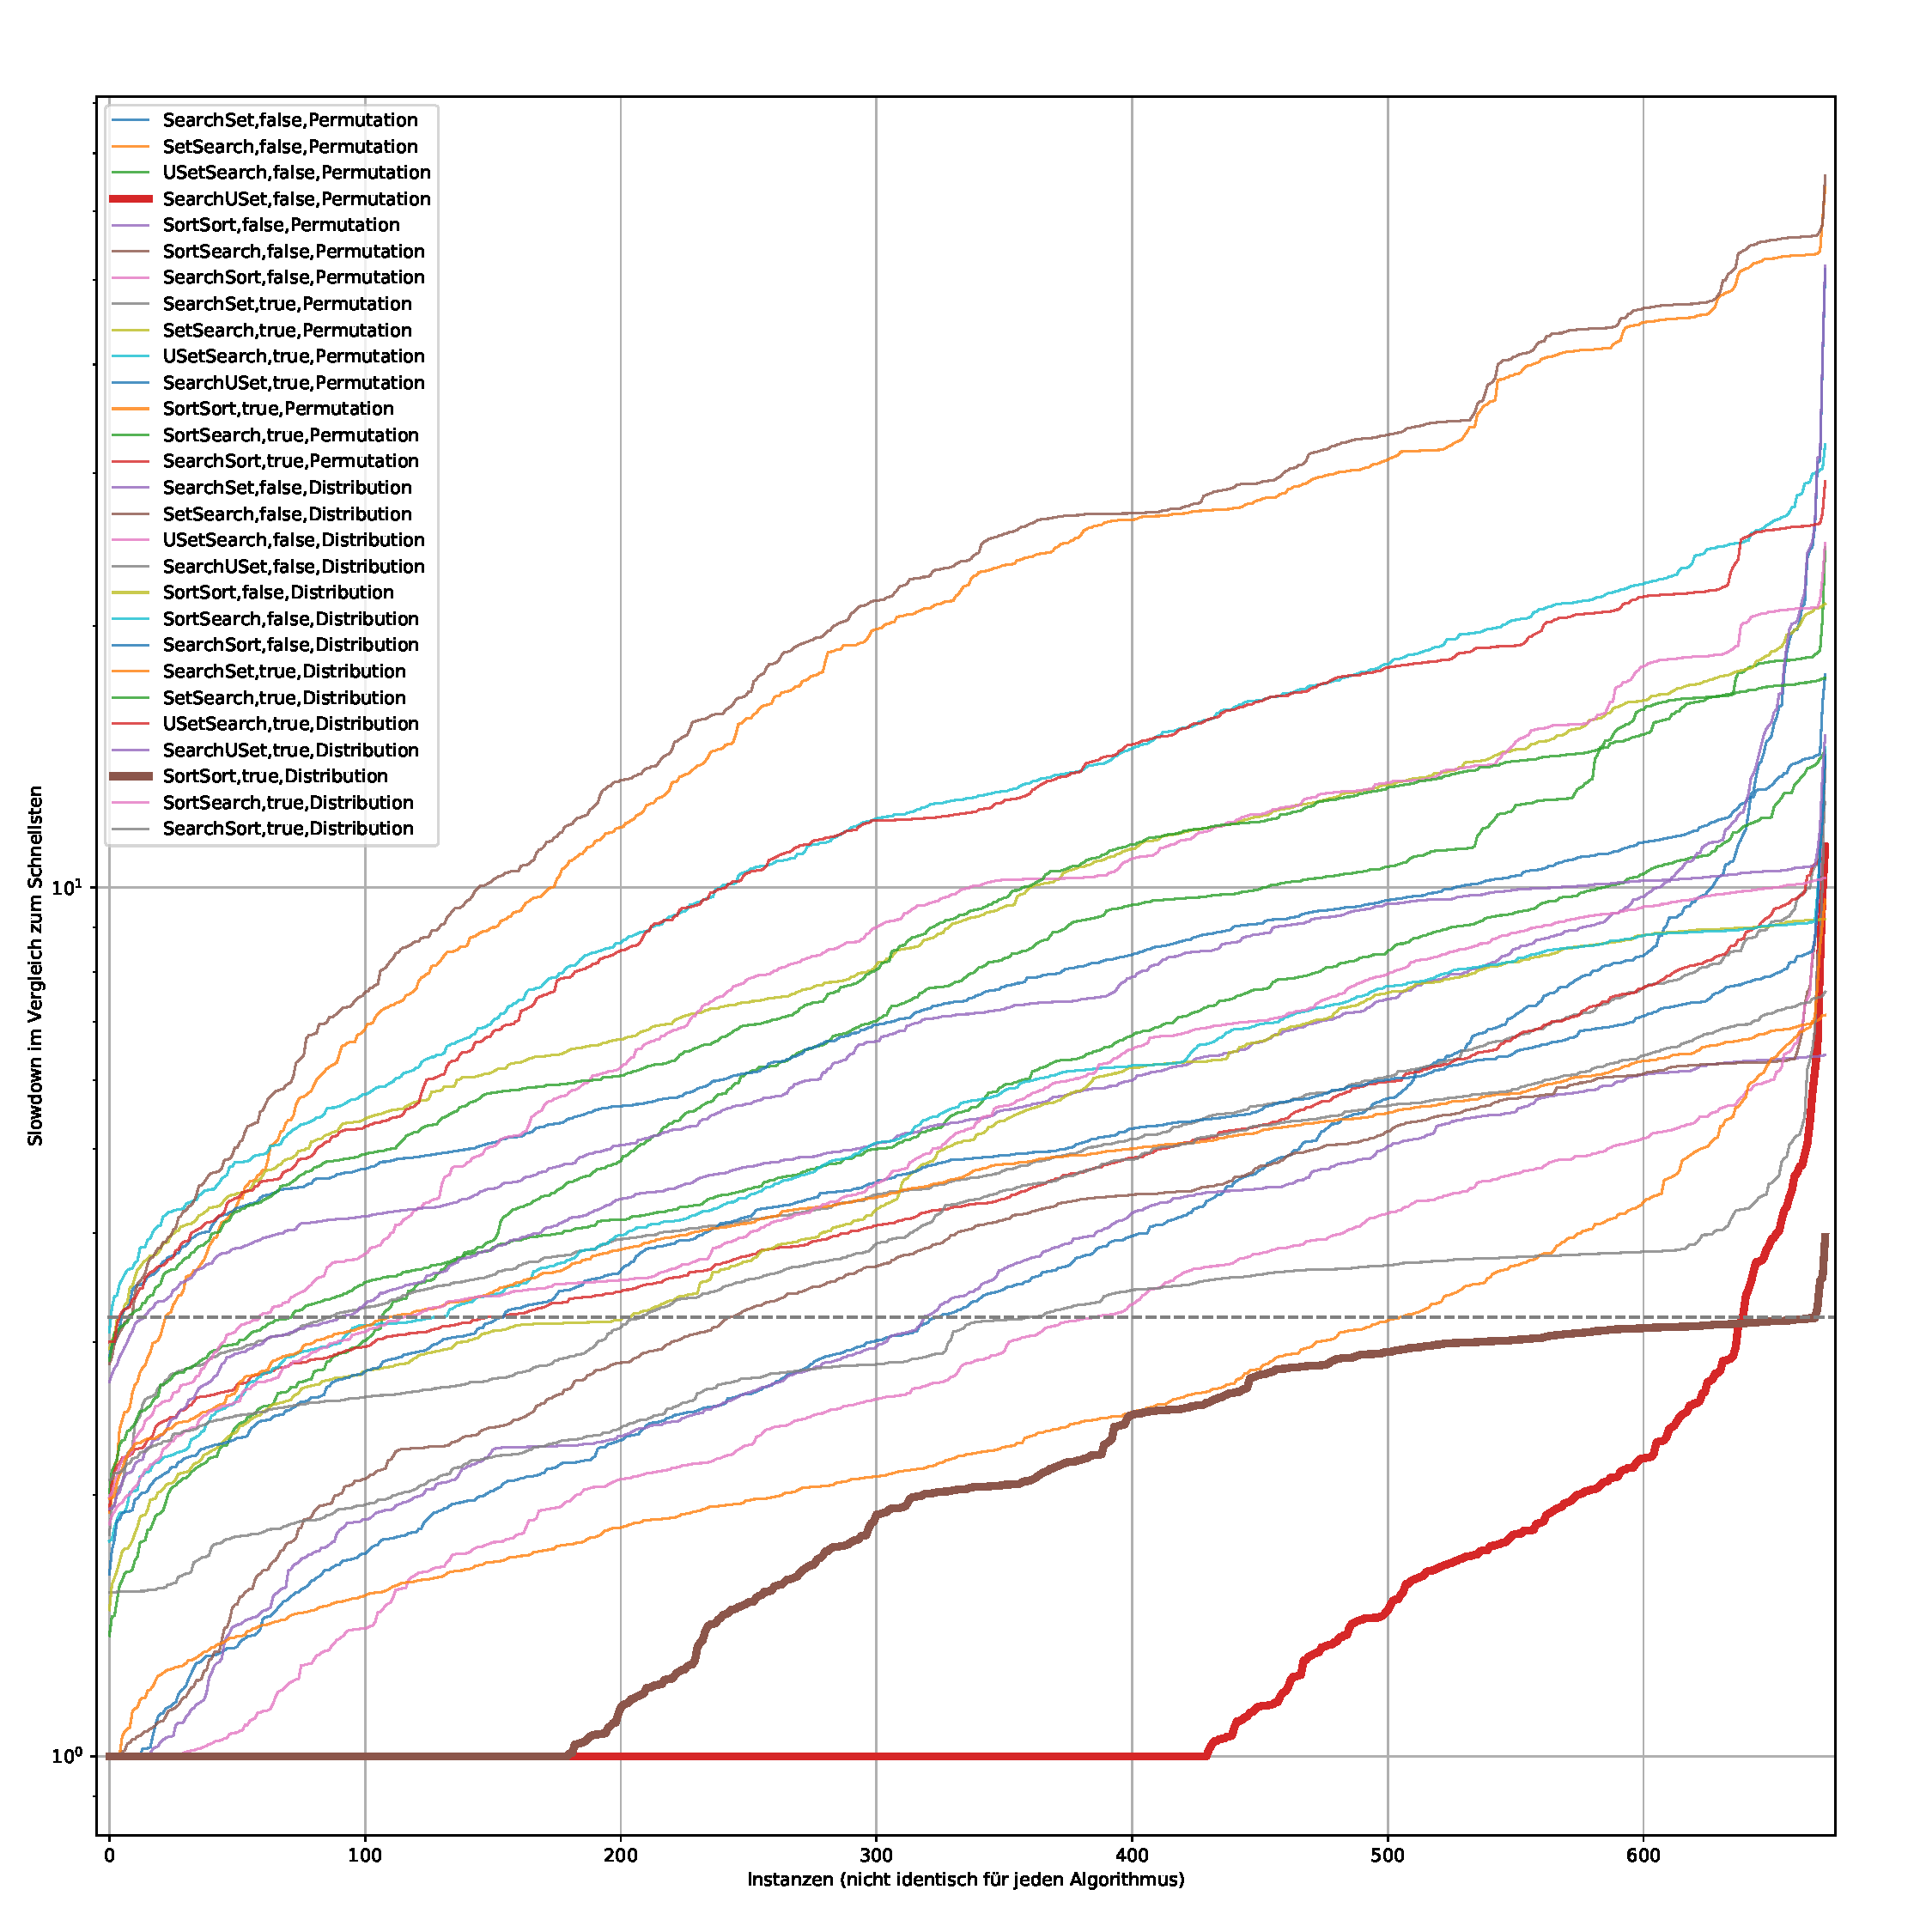
\includegraphics[width = 1\textwidth]{figures/slowdown.pdf}
	\caption[Slowdown der einzelnen Varianten im jeweiligen Vergleich zur Variante mit der geringsten Laufzeit.]
	{Slowdown der einzelnen Varianten im jeweiligen Vergleich zur Variante mit der geringsten Laufzeit. 
	Dabei ist der Wert 3.5 als gestrichelte Linie eingezeichnet}
	\label{fig:messung_slowdown}
\end{figure}
Um diesen Plot zu erstellen, wurde jede Variante einzeln betrachtet.
Dann wird für jede Instanz bestimmt, welche Variante die kürzeste Laufzeit hat und der Quotient
aus dieser Laufzeit und der Laufzeit der betrachteten Variante berechnet. Dieses Verhältnis wird als Slowdown
bezeichnet und gibt an, um welchen Faktor die Variante langsamer als die schnellste ist. Die Slowdowns
zu jeder Instanz werden schließlich aufsteigend sortiert und als Kurve in den Plot eingefügt.
Da die Slowdowns jedoch für jede Variante unabhängig voneinander sortiert werden, geht dadurch 
die Ordnung über die Instanzen verloren. Somit entspricht eine Stelle auf der horizontalen Achse 
nicht für jede Variante der gleichen Instanz. Einen \glqq guten\grqq{} Algorithmus erkennt man in diesem
Plot, wenn die entsprechende Kurve lange nahe der eins verläuft.
\\

Dieser Plot legt ebenfalls nahe, sich auf die beiden Varianten (\SeaUSet, \false, \perm) und 
(\SorSor, \true, \distr) zu konzentrieren, da die beiden Kurven am wenigsten stark wachsen und damit 
die Slowdowns vergleichsweise klein sind. Jedoch lässt sich auch hier nicht bestimmen, welche der beiden
Varianten die bessere ist. Ein Vorteil von (\SeaUSet, \false, \perm) ist, 
dass die Methode auf den meisten Instanzen einen Slowdown
von eins hat ---was wir ja auch schon in Abbildung \ref{fig:messung_counting} gesehen haben---
und damit langsamer anwächst. Ein Nachteil liegt aber darin, dass der Slowdown für manche Instanzen
eine Größe von bis zu 10 erreicht, während der Slowdown von  (\SorSor, \true, \distr) durch den maximalen
Wert von 3.5 beschränkt ist.
\newpage
Dieser Nachteil spiegelt sich ebenfalls in Abbildung \ref{fig:messung_mean} wieder. Für diesen Plot
wurde über alle Instanzen für jede Variante jeweils die mittlere Laufzeit bestimmt. Obwohl
es nicht in den meisten Fällen die schnellste Variante ist, hat (\SorSor, \true, \distr) die 
kleinste mittlere Laufzeit mit rund 38 Millisekunden. Auf Platz zwei folgt
(\SeaUSet, \false, \perm) mit etwa 64 Millisekunden, was schon einer Abweichung von ungefähr 60\% entspricht.
Auch in diesem Plot sieht man deutlich, dass es sich nicht lohnt, noch weitere Varianten zu betrachten. Zwar hat 
auch (\SorSor, \true, \perm) eine mittlere Laufzeit, 
die annähernd so groß ist wie die Laufzeit von (\SeaUSet, \false, \perm), aber 
auch diese kommt nicht an die Schnellste heran. Alle anderen Varianten 
haben eine deutlich größere mittlere Laufzeit.
\begin{figure}
\centering
	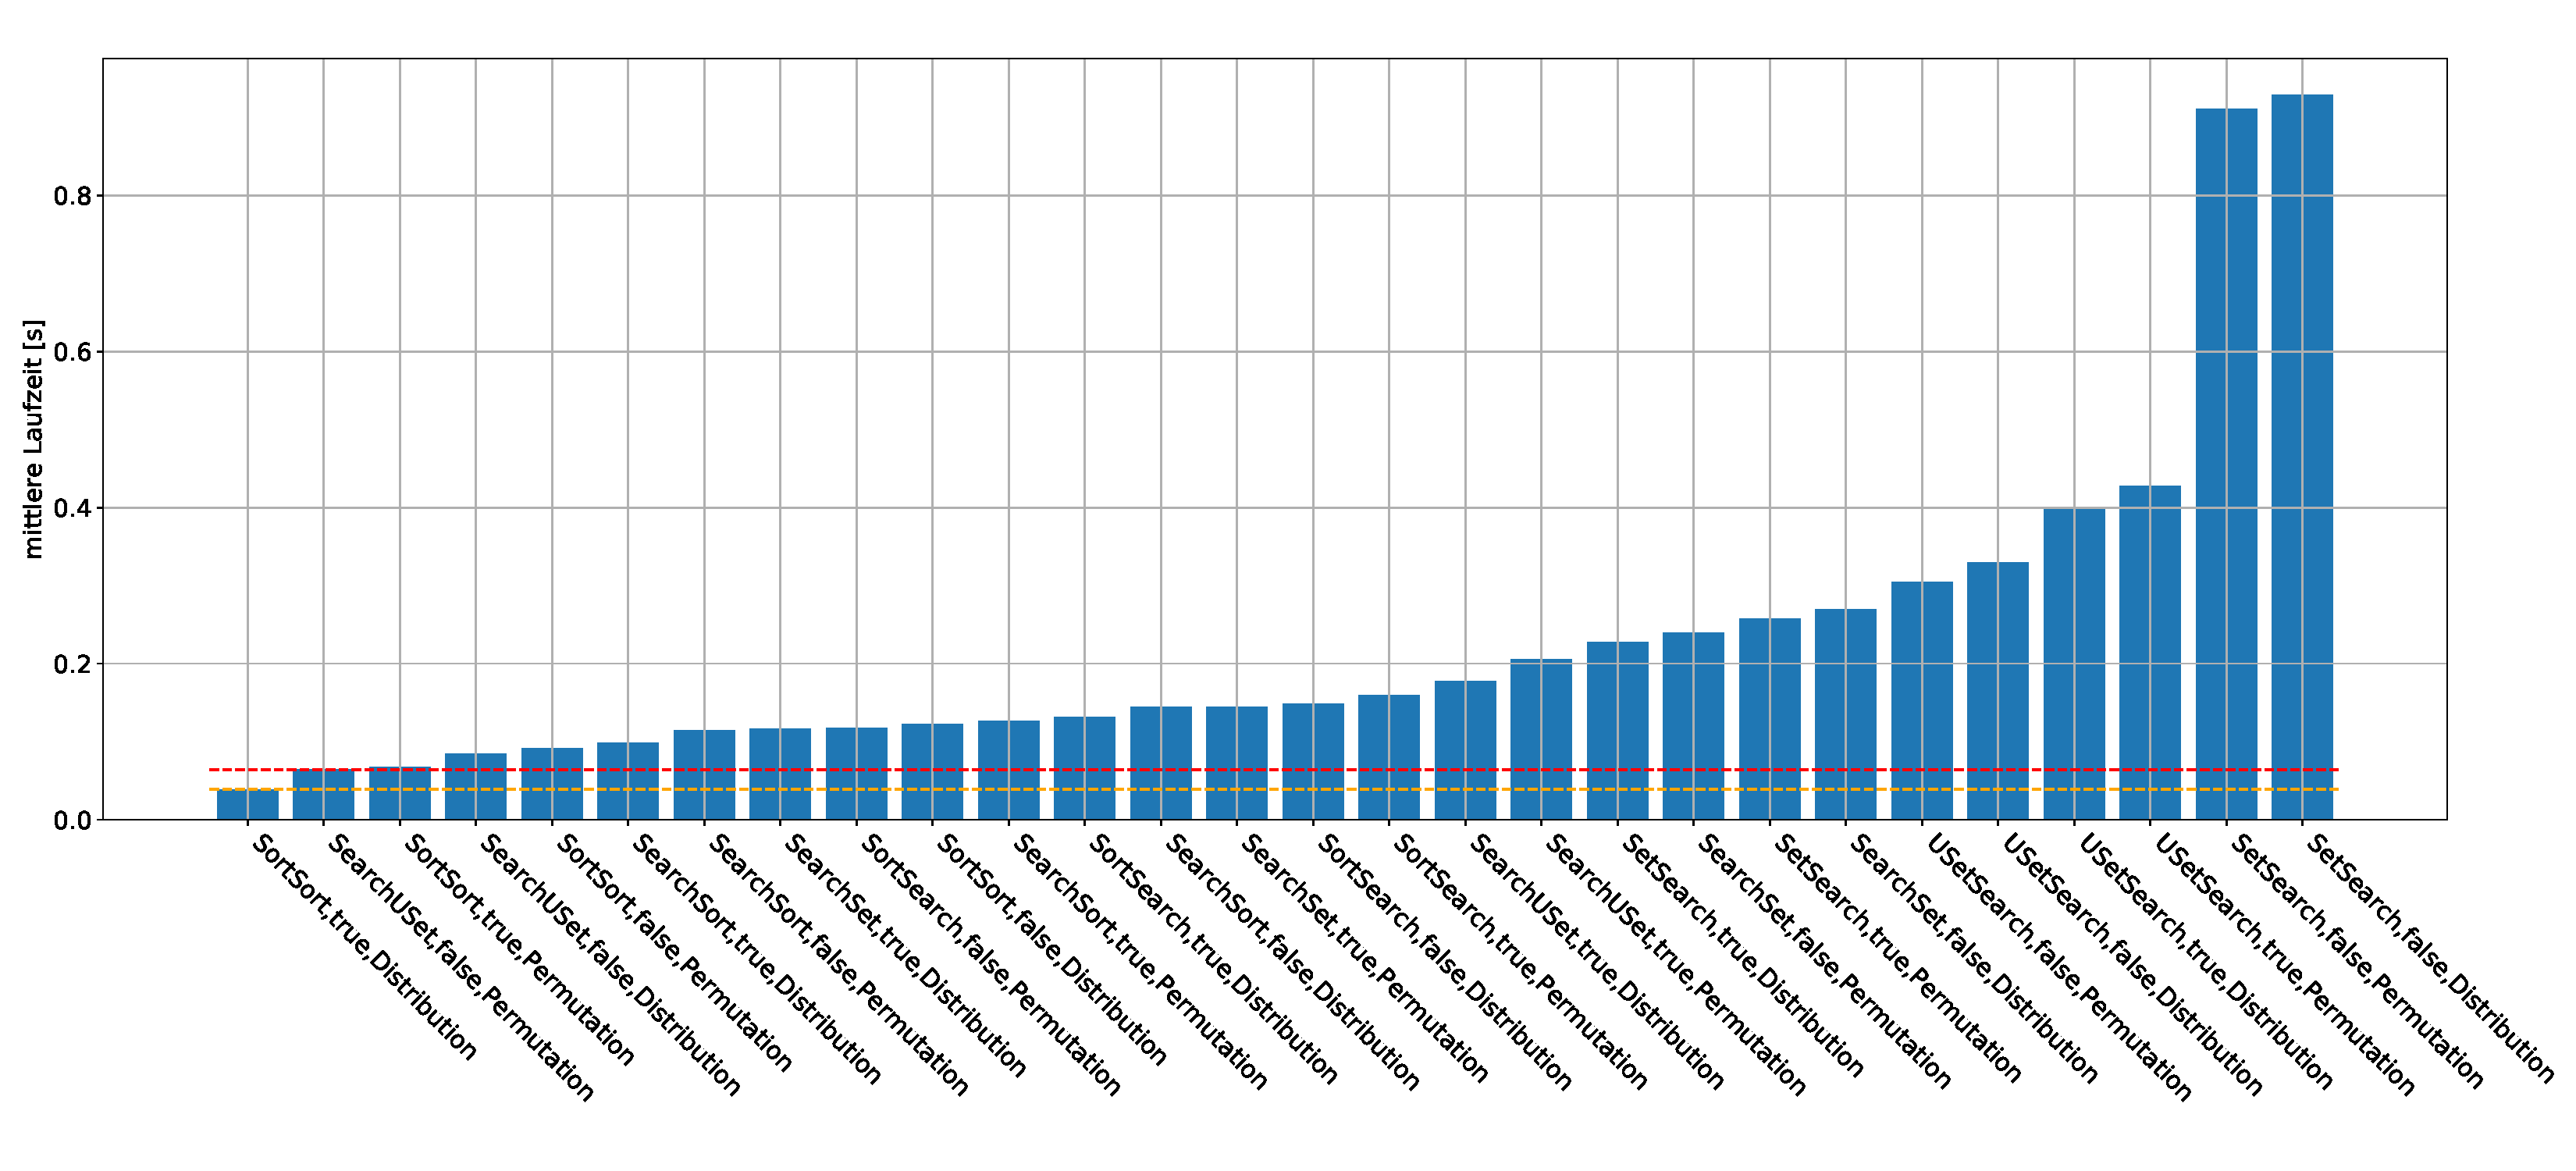
\includegraphics[width = \textwidth]{figures/mean.pdf}
	\caption{Mittlere Laufzeiten der Varianten über allen Instanzen}
	\label{fig:messung_mean}
\end{figure}
\\

Abschließend betrachten wir noch die zwei ausgewählten Varianten im direkten Vergleich. Hierzu wurden
in Abbildung \ref{fig:messung_small} auf der horizontalen Achse die getesteten Instanzen aufgetragen
und dazu die jeweiligen Laufzeiten von (\SorSor, \true, \distr) und (\SeaUSet, \false, \perm) als Punkte
eingezeichnet. 
Man sieht dabei, dass sich die Laufzeiten in den meisten Instanzen nicht so stark unterscheiden.
Dies sind vor allem die Instanzen, bei denen der Unterschied zwischen \la{} und \sm{} nicht so groß ist.
In den Instanzen, in denen sich die Werte für \sm{} und \la{} stark unterscheiden, ist jedoch ein 
deutlicher Vorteil von (\SorSor, \true, \distr) zu erkennen. Auch bei den \glqq großen\grqq{} Instanzen
mit Werten von $\text{\sm{}}> 500.000$ hat diese Variante einen deutlichen Laufzeitvorteil.
Auf der Instanz (4.194.304, 4.194.304, 75) beispielsweise hat (\SeaUSet, \false, \perm) eine Laufzeit
von circa 1,628 Sekunden, während (\SorSor, \true, \distr) nur etwa 0,146 Sekunden benötigt. Der Slowdown
beträgt für diese Instanz also in etwa einem Wert von 11. 
\begin{figure}
\centering
	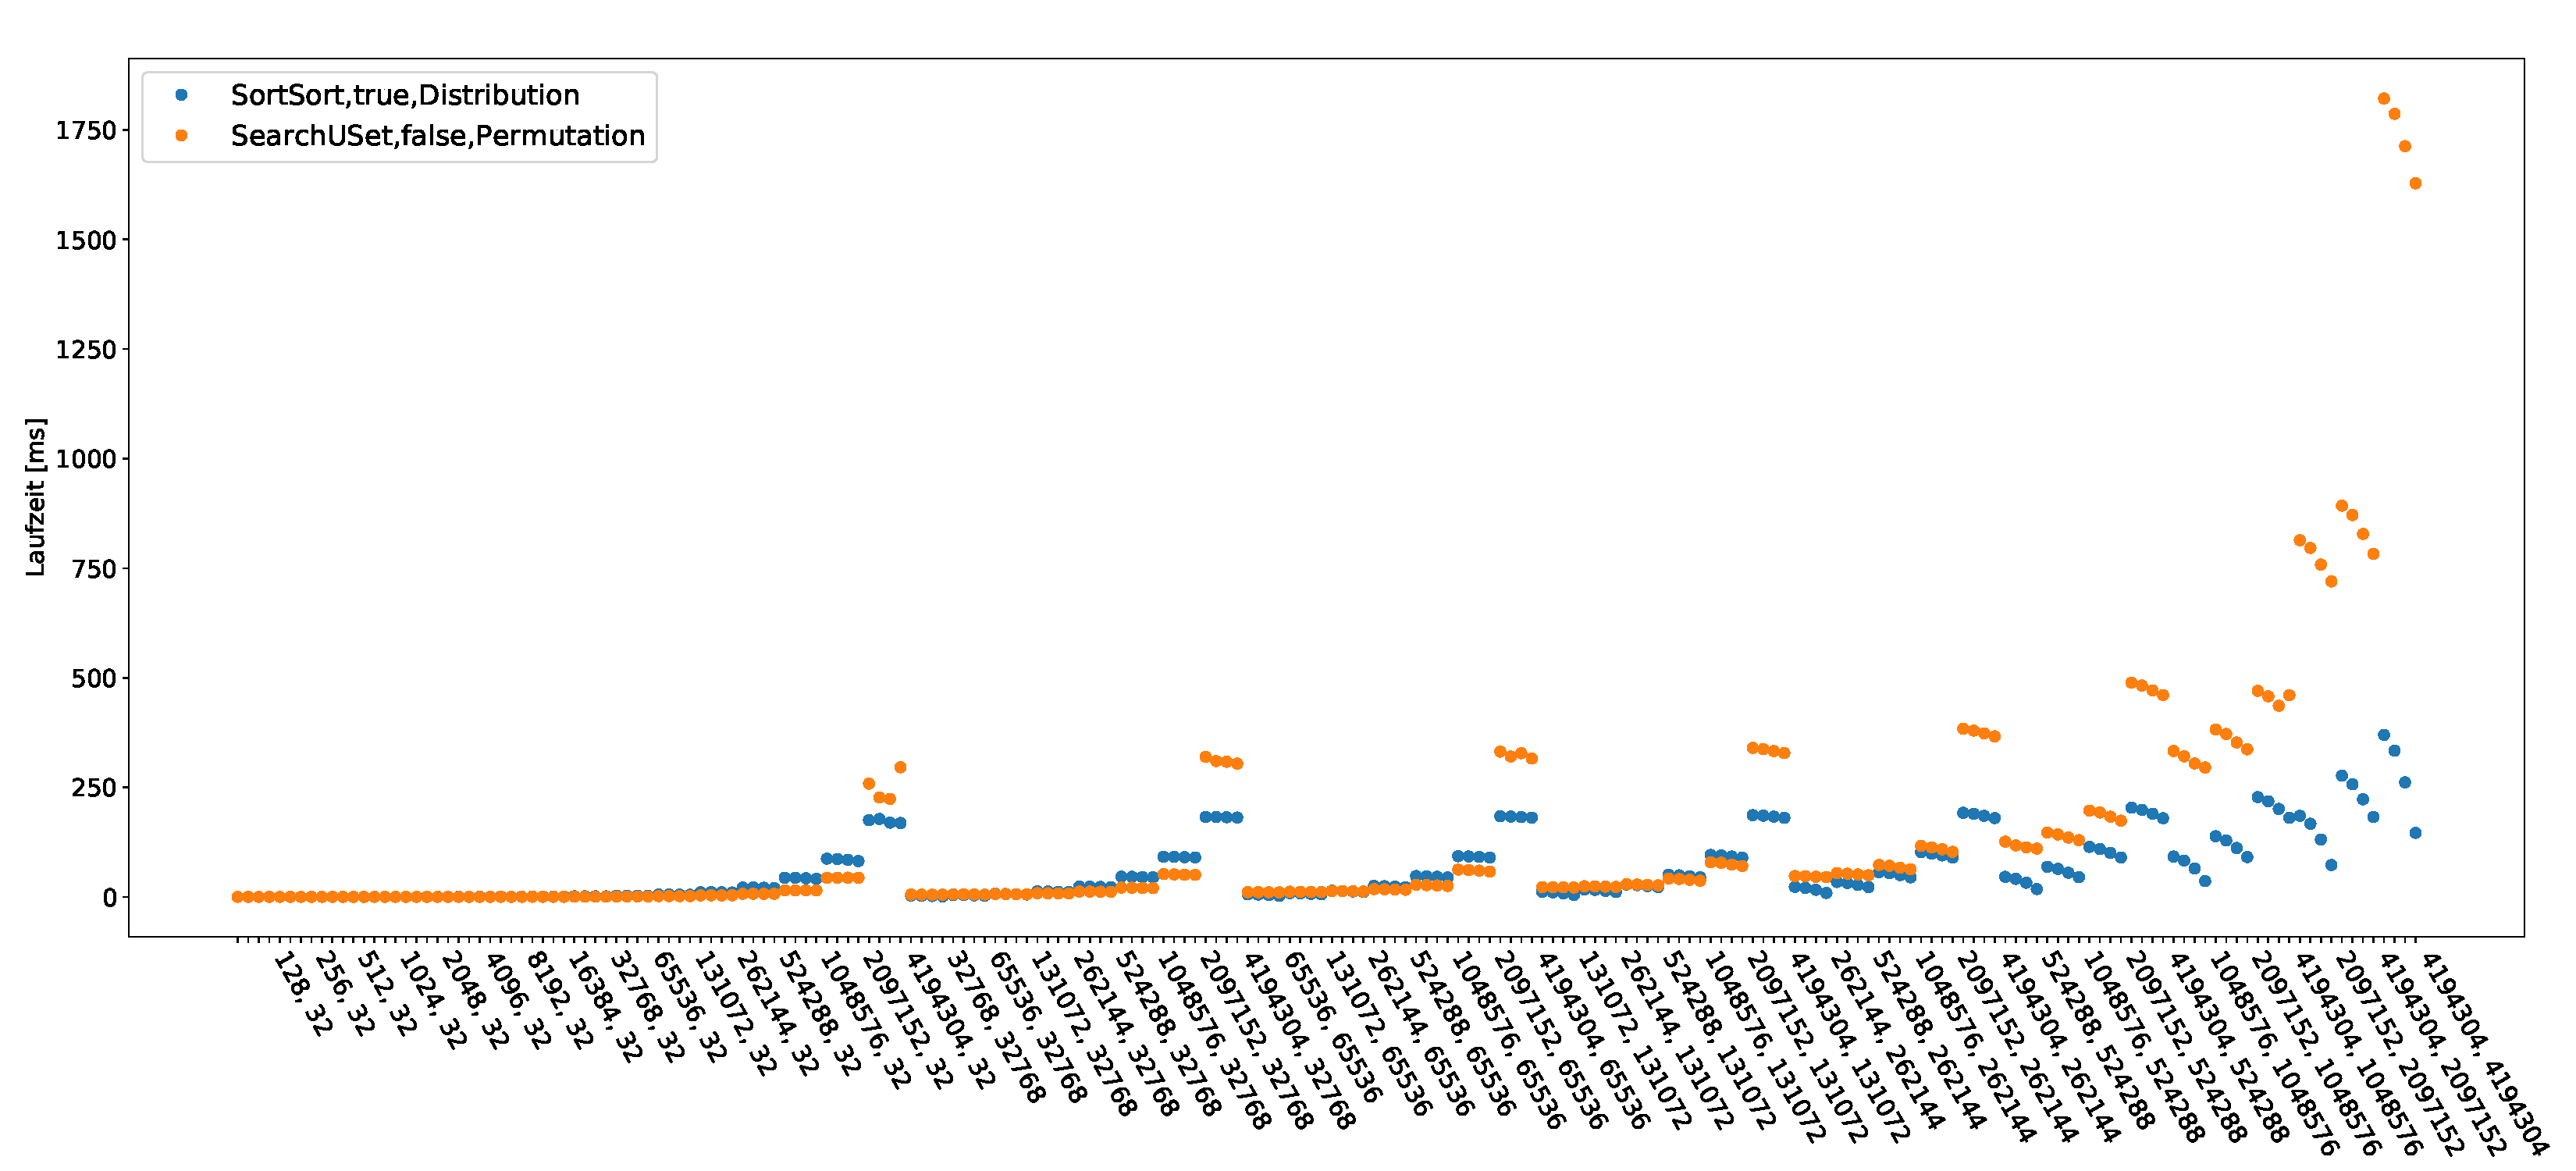
\includegraphics[width = \textwidth]{figures/small_aufsteigend.pdf}
	\caption[Laufzeitvergleich der zwei besten Varianten auf ausgewählten Instanzen] {Vergleich der Laufzeiten der zwei besten Varianten auf ausgewählten Instanzen.
			Die Instanzen sind nach aufsteigenden Werten für \sm{} sortiert. Aus Gründen der Übersichtlichkeit
wird bei  der Beschriftung der Instanzen der Teil \fr{} weggelassen, die Instanzen werden 
nur mit \la{}, \sm{} bezeichnet. Weiterhin wurden der
Übersichtlichkeit wegen die Instanzen aus dem Bereich $32 < \text{\sm}  <32768$ ausgelassen, da sie das gleiche
Bild wie die üblichen Instanzen zeigen.}
	\label{fig:messung_small}
\end{figure}

%%%%%%%%%%%%%%%%%%%%%%%%%%%%%%%%%%%%%%%%%%%%%%%%%%%%%%%%%%%%%%%%%%%%%%%%
%%%%%% Diskussion
%%%%%%%%%%%%%%%%%%%%%%%%%%%%%%%%%%%%%%%%%%%%%%%%%%%%%%%%%%%%%%%%%%%%%%%%

\section{Diskussion der Ergebnisse}
Es gilt zu überprüfen, ob die ermittelten Ergebnisse zu erwarten waren, indem wir sie 
mit den asymptotischen Laufzeiten aus der Tabelle \ref{tab:varianten} vergleichen.
Laut den asymptotischen Laufzeiten sollte die Variante mit \SorSor{}, \distr{} und vorsortiert am schnellsten
sein. Dies sieht man auch bei den mittleren gemessenen Laufzeiten aus Abbildung \ref{fig:messung_mean}.
Dabei liegt diese Variante deutlich auf dem ersten Platz. Die dazugehörige Variante mit
der Tausch-Methode \perm{} liegt auf dem dritten Platz, obwohl sie im Vergleich eine der
schlechtesten asymptotischen Laufzeiten hat. Der Grund für diese Diskrepanz 
liegt vermutlich darin, dass diese
asymptotische Laufzeit durch das einmalige Sortieren am Ende der Methode entsteht. 
In anderen Varianten, welche die gleiche asymptotische Laufzeit haben, wird jedoch eventuell häufiger
sortiert oder eine Datenstruktur verwendet, die eine höhere Laufzeit produziert.
\\

Auffällig ist, dass die Varianten mit \USetSea{} jeweils deutlich langsamer sind als die analogen
Varianten, welche \SeaUSet{} verwenden, obwohl die erwarteten asymptotischen Laufzeiten
gleich sind. Dies liegt höchstwahrscheinlich an der
Datenstruktur \texttt{unordered\_set}, einer Hash-Tabelle. Bei dieser Datenstruktur
sind die Laufzeiten stark abhängig vom Füllgrad, also dem Anteil der 
gespeicherten Elemente im Bezug zur Größe der Hash-Tabelle. Da bei \USetSea{} die Elemente
des größeren Arrays in die Hash-Tabelle eingefügt werden, ist der Füllgrad dementsprechend
auch größer, was zu der schlechteren Laufzeit führt.
Im Gegensatz dazu ist die Methode, welche \SeaUSet, \perm{} und keine Vorsortierung verwendet,
die im Mittel zweitschnellste aller gemessenen Varianten, da sich hierbei
weniger Elemente in der Hash-Tabelle befinden und der Füllgrad demnach geringer ist. 
Somit wird auch eher die Laufzeit des Erwartungswerts erreicht.
\\

Mit einem ähnlichen Argument lassen sich auch die schlechten Laufzeiten 
der Varianten, welche \SetSea{} verwenden, erklären. Hierbei wird ebenfalls das größere
Array in die Datenstruktur eingefügt, was zu der schlechteren Laufzeit führt.  
Dabei fällt jedoch noch auf, dass vor allem die Varianten, 
bei welchen nicht vorsortiert wird, die mit Abstand längsten Laufzeiten besitzen. Als Begründung 
dient hier, dass beim Erstellen des Binärbaums für jeden Knoten, welcher eingefügt wird,
eine Speicherallokation ausgeführt wird, was sehr laufzeitintensiv ist. Ist die
Eingabe bereits sortiert, kann dies von der Implementierung des Binärbaums ausgenutzt werden.
\\

Insgesamt wirken die gemessenen mittleren Laufzeiten 
also plausibel.



%%%%%%%%%%%%%%%%%%%%%%%%%%%%%%%%%%%%%%%%%%%%%%%%%%%%%%%%%%%%%%%%%%%%%%%%
%%%%%% Fazit
%%%%%%%%%%%%%%%%%%%%%%%%%%%%%%%%%%%%%%%%%%%%%%%%%%%%%%%%%%%%%%%%%%%%%%%%

\section{Auswahl der besten Variante}
\label{sec:entscheidung}
Abschließend muss anhand der Messdaten entschieden werden, welche Variante zum Einsatz für
einen \ct{} am besten geeignet ist.
Zusammenfassend haben wir im Abschnitt \ref{ref:auswertung} festgestellt, 
dass hierfür nur die Varianten (\SorSor, \true, \distr) und (\SeaUSet, \false, \perm) zur Auswahl stehen.
Während die eine Variante am häufigsten die geringste Laufzeit hat, liegt die andere 
bei der durchschnittlichen Laufzeit weiter vorne. Dies liegt vor allem daran, dass sich 
die Laufzeiten bei den Instanzen, auf denen (\SeaUSet, \false, \perm) \glqq gewinnt\grqq{}, kaum unterscheiden.
Unter den anderen Instanzen gibt es jedoch welche, bei denen (\SorSor, \true, \distr) bis auf einen
Faktor von circa 11 schneller ist.
\\

Um ein bestmögliches Laufzeitverhalten für einen \ct{} zu erreichen, könnte man auf die Idee kommen, 
beide Varianten zusammen zu nutzen
und dabei eine Heuristik entwickeln, die jeweils angibt,
auf welcher Instanz man welche Variante verwenden sollte. Somit würde bei jedem \ct{} abhängig von 
der Eingabe, also den Nachbarschaften, entschieden werden, welche der beiden Instanzen man benutzt. 
Das Problem dabei liegt jedoch darin, dass bei diesen Varianten einmal die Vorsortierung
genutzt wird und einmal nicht. Dies ist allerdings nicht beides gemeinsam möglich. Entweder hält man die
Nachbarschaften immer sortiert, oder nicht. Man muss sich also für eine Möglichkeit dieser
Variante  entscheiden. Dadurch ändert sich dann aber zwangsläufig  eine der beiden anderen Varianten. 
Entscheidet man sich die Nachbarschaften sortiert zu halten, würde (\SeaUSet, \false, \perm) zu (\SeaUSet, \true, \perm){}
werden, andernfalls würde sich (\SorSor, \true, \distr) zu (\SorSor, \false, \distr) verändern.
Diese beiden \glqq veränderten\grqq{} Varianten haben aber jeweils deutlich schlechtere Laufzeiten
als die ursprünglichen.
\\

Es ist also nicht sinnvoll möglich, die beiden Varianten miteinander zu kombinieren. Wir müssen uns
also auf eine Variante festlegen. Dies ist die Variante (\SorSor, \true, \distr), da sie im Vergleich zur
Alternative ---wie schon beschrieben---
in kaum einer Instanz eine wesentlich schlechtere Laufzeit hatte, jedoch auf manchen Instanzen wesentlich
bessere Laufzeiten. Außerdem ist es die Variante mit der geringsten mittleren Laufzeit. 
Ein Vorteil dieser Variante neben der Laufzeit liegt noch in der Einfachheit. So werden
lediglich die beiden Arrays sortiert und linear durchlaufen. Es muss keine weitere Datenstruktur
erstellt werden ---wie bei der anderen Variante das \texttt{unordered\_set}--- und damit wird
auch kein zusätzlicher Speicherplatz verbraucht.


%%%%%%%%%%%%%%%%%%%%%%%%%%%%%%%%%%%%%%%%%%%%%%%%%%%%%%%%%%%%%%%%%%%%%%%%
%%%%%% Fazit
%%%%%%%%%%%%%%%%%%%%%%%%%%%%%%%%%%%%%%%%%%%%%%%%%%%%%%%%%%%%%%%%%%%%%%%%


\section{Vergleich zum Standard \cb{}}
\label{kap:result}
In einem letzten Experiment wird geprüft, wie sich die Laufzeit der bipartiten \gc{}
Variante, sowohl im parallelen als auch im sequenziellen Fall,
 im Vergleich zum \cb{} auf massiven Graphen verhält.
\\

Dazu werden wir verschiedene Test-Instanzen erstellen.
Als Grundlage dient ein Netflix-Datensatz\cite{kaggle}, welcher Nutzer- und Film-Knoten enthält, 
wobei eine gerichtete Kante von einem Film zu einem Nutzer gezogen wird, wenn dieser den 
Film gut bewertet hat. Damit liegen die Film-Knoten in einer Partitionsklasse und 
die Nutzer-Knoten in der anderen.
Aus diesem Graph werden drei Subgraphen erstellt, wobei jeweils 1000, 10.000 und 100.000  zufällige
Nutzer-Knoten ausgewählt werden und deren vollständige Nachbarschaft hinzugefügt wird.
Für jeden dieser drei Graphen gibt es zwei Varianten. Der Unterschied
zwischen den beiden Varianten liegt darin, welche der beiden Partitionsklassen aktiv sind, 
also auf welcher Partitionsklasse die \ct{e} ausgeführt werden.
Somit ergeben sich sechs Instanzen. 
\\

Auf diesen wird 
die in dieser Arbeit erarbeite bipartite Version des \gc{} ausgeführt. Dazu müssen die
einzelnen Graphen jedoch jeweils in einen ungerichteten Graph transformiert werden.
\\

Als Vergleich verwenden wir an dieser Stelle nicht 
den Standard \gc{} Algorithmus. Dies liegt daran, 
dass bei diesem Algorithmus auf bipartiten Graphen die Eigenschaft der
Bipartitheit verletzt werden könnte und zusätzlich viele unnötige \ct{e} ausgeführt werden. 
Auf einem bipartiten Graphen liegen in der disjunkten Nachbarschaft zweier Knoten, 
welche nicht aus der gleichen Partitionsklasse stammen, entweder keine Knoten,
 oder die beiden Knoten selbst. 
Führt man nun ein \ct{} auf diesen beiden Knoten aus, verändert sich entweder (im Falle einer leeren disjunkten
Nachbarschaft) nichts
oder es könnte passieren, dass ein Knoten sich selbst in seine Nachbarschaft getauscht bekommt.
Damit hätte dieser Knoten eine Kante zu sich selbst, was es jedoch auf bipartiten Graphen nicht 
geben darf.
\\

Deshalb wird als Vergleich der Standard \cb{} Algorithmus \cite{DBLP:conf/esa/CarstensH0PTW18}
sowohl auf den ungerichteten als auch auf den gerichteten Graphen ausgeführt.
Um die Probleme, welche wir für den \gc{} Algorithmus beschrieben haben, zu umgehen, 
führen wir die einzelnen \ct{e} ausschließlich auf Knoten einer Partitionsklasse aus.
\\

Um zusätzlich zu sehen, wie stark die Parallelisierung die Laufzeit des bipartiten
\gc{} beeinflusst, werden wir weiterhin eine sequenzielle Variante des bipartiten \gc{} 
untersuchen.
\\

Alle vier beschriebenen Varianten werden nacheinander auf dem gleichen Prozessor ausgeführt, welcher 8
Kerne mit Hyperthreading besitzt. Es werden bei jeder Variante insgesamt 10 Globale Tausche vorgenommen.
In Abbildung \ref{fig:speedup_komplett} sind die gemessenen Laufzeiten in Form
eines Balkendiagramms grafisch dargestellt.
Um eventuelle Messfehler zu verringern, wurde jede Messung zehnmal 
wiederholt. Dabei sind jeweils die Mittelwerte der Messungen aufgetragen.
\\

Dabei fällt auf, dass sich die Laufzeiten von \cb{} und bipartitem \gc{} auf den
Instanzen mit über 100.000 Knoten deutlich unterscheiden. Auf diesen Instanzen erreicht
der bipartite \gc{} einen Speedup von bis zu 17. 
Während die Laufzeit der angepassten \cb{} Variante auf dem gerichteten Graphen in etwa 9 Sekunden
und auf dem ungerichteten etwa 10,5 Sekunden beträgt, liegt sie beim bipartiten \gc{} bei lediglich 
0,6 Sekunden. Dies entspricht ---auf dieser Instanz---  einem Speedup von ungefähr 17.
Auf den Instanzen mit ungefähr 25.000 Knoten wird ein Speedup zwischen 3 und 5 erreicht.
Bei den kleineren, etwa 10.000 Knoten umfassenden Instanzen, besitzt die \cb{} Implementierung jedoch 
eine leicht geringere Laufzeit.
\\

Für die sequentielle Variante des \gc{} lässt sich sagen, dass die Laufzeiten auf jeder Instanz um
einen annähernd konstanten Faktor geringer sind, als die von den beiden \cb{} Varianten. 
Dies liegt vor allem daran, 
dass ein einzelner \ct{} auf bipartiten Graphen einfacher aufgebaut ist, als auf allgemeinen Graphen.
Auch die verbesserte Datenstruktur im bipartiten \gc{} führt zu der geringeren Laufzeit.
Während im bipartiten \gc{} durch das Tauschen der Nachbarschaft direkt die Datenstruktur
aktualisiert wird, müssen beim \cb{} noch Kanten zur Adjazenzlistendarstellung hinzugefügt, 
beziehungsweise entfernt, werden.
Auf der größten Instanz wird somit ein Speedup von ungefähr 2 erreicht.
Im Vergleich mit der parallelen Version des bipartiten \gc{}, besitzt diese in den meisten Fällen
eine geringere Laufzeit, als die sequenzielle Variante. Dies liegt an der Parallelisierung und
war damit zu erwarten. Einzig auf den Instanzen mit lediglich 10.000 Knoten, hat die sequenzielle
Variante eine geringere Laufzeit. Dies liegt vermutlich an einem Overhead, der durch die Koordination
der einzelnen parallelen Threads durch OpenMP entsteht.
\\

Insgesamt fällt jedoch auf, dass die Laufzeiten bei wachsender Größe für die \cb{}
Variante stark ansteigen, wobei die Laufzeit vom parallelen bipartiten \gc{} im Vergleich dazu
relativ konstant bleiben.
\begin{figure}
\centering
	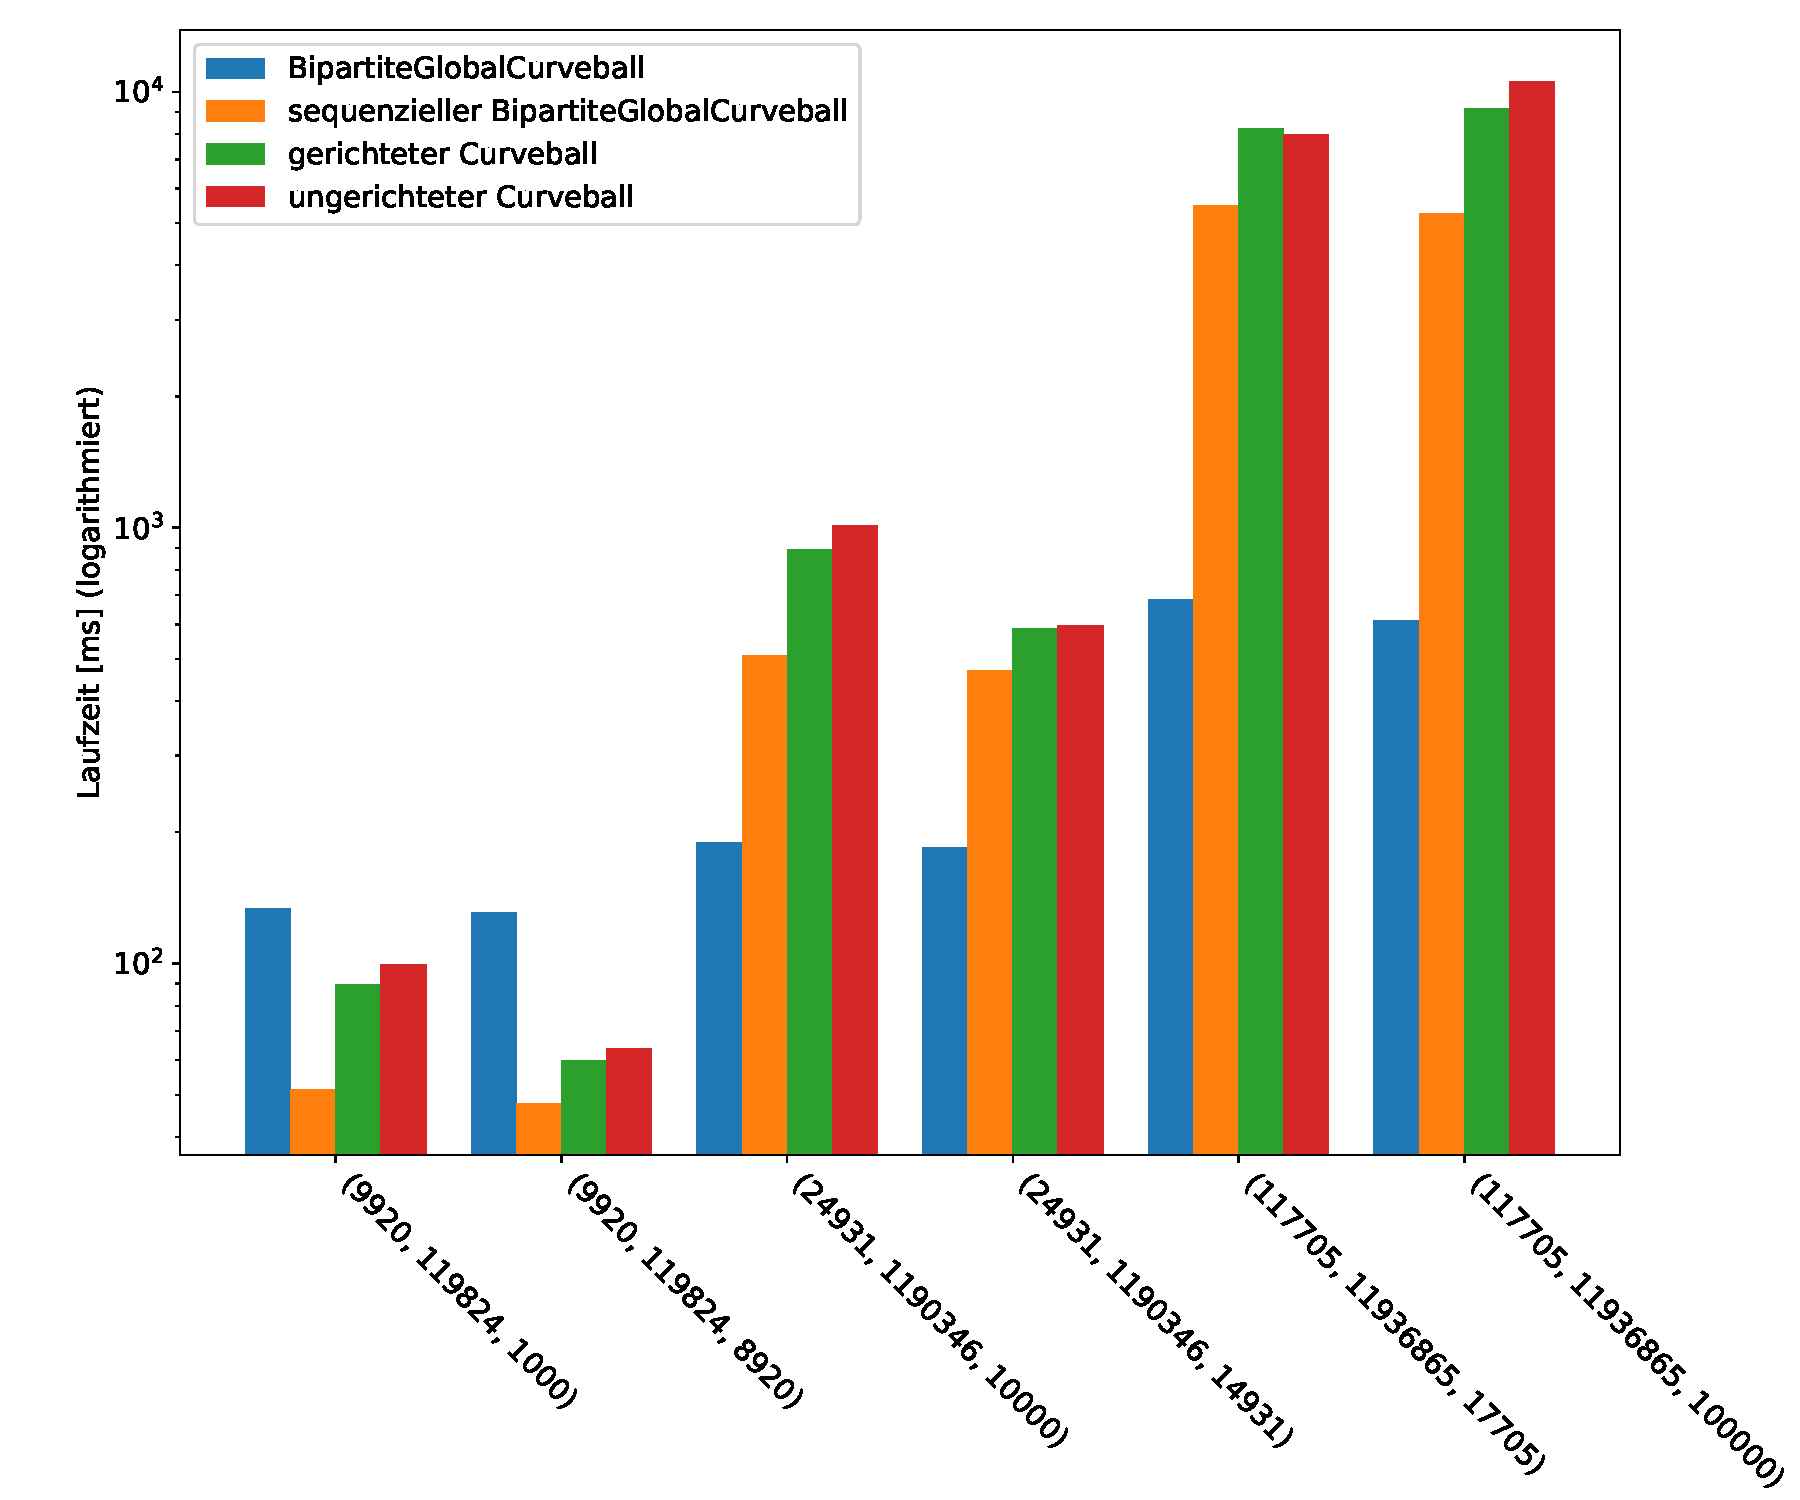
\includegraphics[width = 0.8\textwidth]{figures/speedup.pdf}
	\caption[Laufzeitvergleich von bipartitem \gc{} und einer abgeänderten Variante von \cb{}]{Laufzeitvergleich von bipartitem \gc{} und der abgeänderten Version des \cb{s}.{}
	Auf der horizontalen Achse sind die einzelnen Instanzen als Tripel aufgetragen.
Die erste Stelle steht dabei für die Knotenanzahl des Graphen, 
die zweite Stelle für die Anzahl an Kanten und die dritte für die Anzahl der Knoten aus 
der aktiven Partition.}
	\label{fig:speedup_komplett}
\end{figure}


%\begin{itemize}

%\item Versuche beschreiben. Aufbau, was warum wie wo?
%\item \red{\Large was wurde erwartet, wie passt das ergebnis dazu? was bedeutet es?}
%\item google Test/ google benchmark
%\item
%bestimmung der schnellsten Varianten..\\
%-- disjoint neighbors\\
%-- trade\\
%-- auf welcher Maschine? gluten\\
%plots\\



%\end{itemize}




%%%%%%%%%%%%%%%%%%%%%%%%%%%%%%%%%%%%%%%%%%%%%%%%%%%%%%%%%%%%%%%%%%%%%%%%
%%%%%   Zusammenfassung
%%%%%%%%%%%%%%%%%%%%%%%%%%%%%%%%%%%%%%%%%%%%%%%%%%%%%%%%%%%%%%%%%%%%%%%%


\chapter{Zusammenfassung}
Zum Abschluss dieser Arbeit





Wir haben gesehen, wie ein \gc{} Tausch und damit auch ein \ct{} aufgebaut ist. 





Verbessern könnte man noch:
verschiedene benchmarks, größere instanzen, einfach mehr...

auf anderem Rechner Architektur/system testen 



Laufzeit Vergleiche...



~\\
\\
\\
\\
\\
was hat das alles gebracht? \\
Algo wird Teil von networkit?\\
ausblick?\\
was könnte man verbessern? mehre tests, andere maschinen
\\
was ist die Laufzeit von einem \gc{} tausch im mittel? für große graphen?

~\\
\\
\\

\red{\Huge TODO:}
\begin{itemize}
	\item Einleitung
	\item Zusammenfassung
	\item \red{\Large \cb{} bezeichnungen undso einheitlich?!}
	\item \red{\Large Anführungszeichen suchen!! + Leerzeichen dahinter}
	\item \red{\huge Laufzeit test für das python ding.. wie schnell funktioniert der algo so?}
	\item \red{wie siehts aus mit der anzahl an global trades?!}
	\item \red{\Large -- Deckblatt?! \\ -- Seitenrand \\ --Zeilenabstand \\ -- Schriftgröße \\ --}
	\item \red{noch was rotes?} \blue{oder was blaues?}
	\item \red{vektor/array?!}
	\item \red{\LaTeX format ?!}
\end{itemize}





%%%%%%%%%%%%%%%%%%%%%%%%%%%%%%%%%%%%%%%%%%%%%%%%%%%%%%%%%%%%%%%%%%%%%%%%
%%%%%   bibliography
%%%%%%%%%%%%%%%%%%%%%%%%%%%%%%%%%%%%%%%%%%%%%%%%%%%%%%%%%%%%%%%%%%%%%%%%


\bibliography{quellen}
\bibliographystyle{plain}


%%%%%%%%%%%%%%%%%%%%%%%%%%%%%%%%%%%%%%%%%%%%%%%%%%%%%%%%%%%%%%%%%%%%%%%%
%%%%%   Abbildungsverzeichnis / Tabellenverzeichnis
%%%%%%%%%%%%%%%%%%%%%%%%%%%%%%%%%%%%%%%%%%%%%%%%%%%%%%%%%%%%%%%%%%%%%%%%


\listoffigures{}
\listoftables{}


\end{document} 
